\section{主要功能介绍}
该系统的主要功能有信息查询、产品添加、零件添加、BOM表显示和用户认证。具体功能架构如图\ref{fig:function}所示:
\begin{figure}[H]
\centering
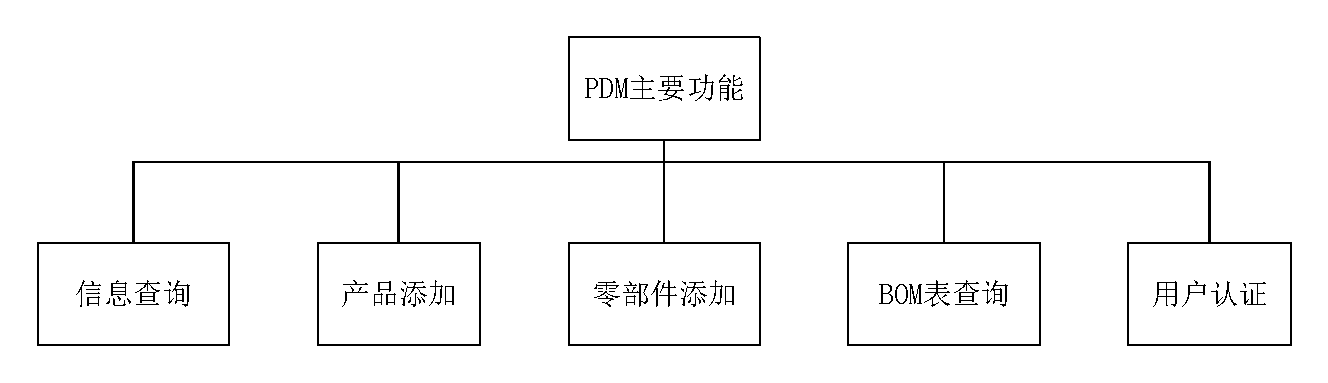
\includegraphics[width=0.9\linewidth]{figure/function.pdf}
\caption{PDM主要功能}
\label{fig:function}
\end{figure}

此外支持对数据汽车产品及零件的查询支持简单查询和高级查询;支持汽车附属零件信息的显示;支持对汽车产品及其零部件的修改和删除;支持通过BOM表显示整个PDM数据库的数据结构。

PDM系统的主界面如图\ref{fig:index1}所示。
\begin{figure}[H]
\centering
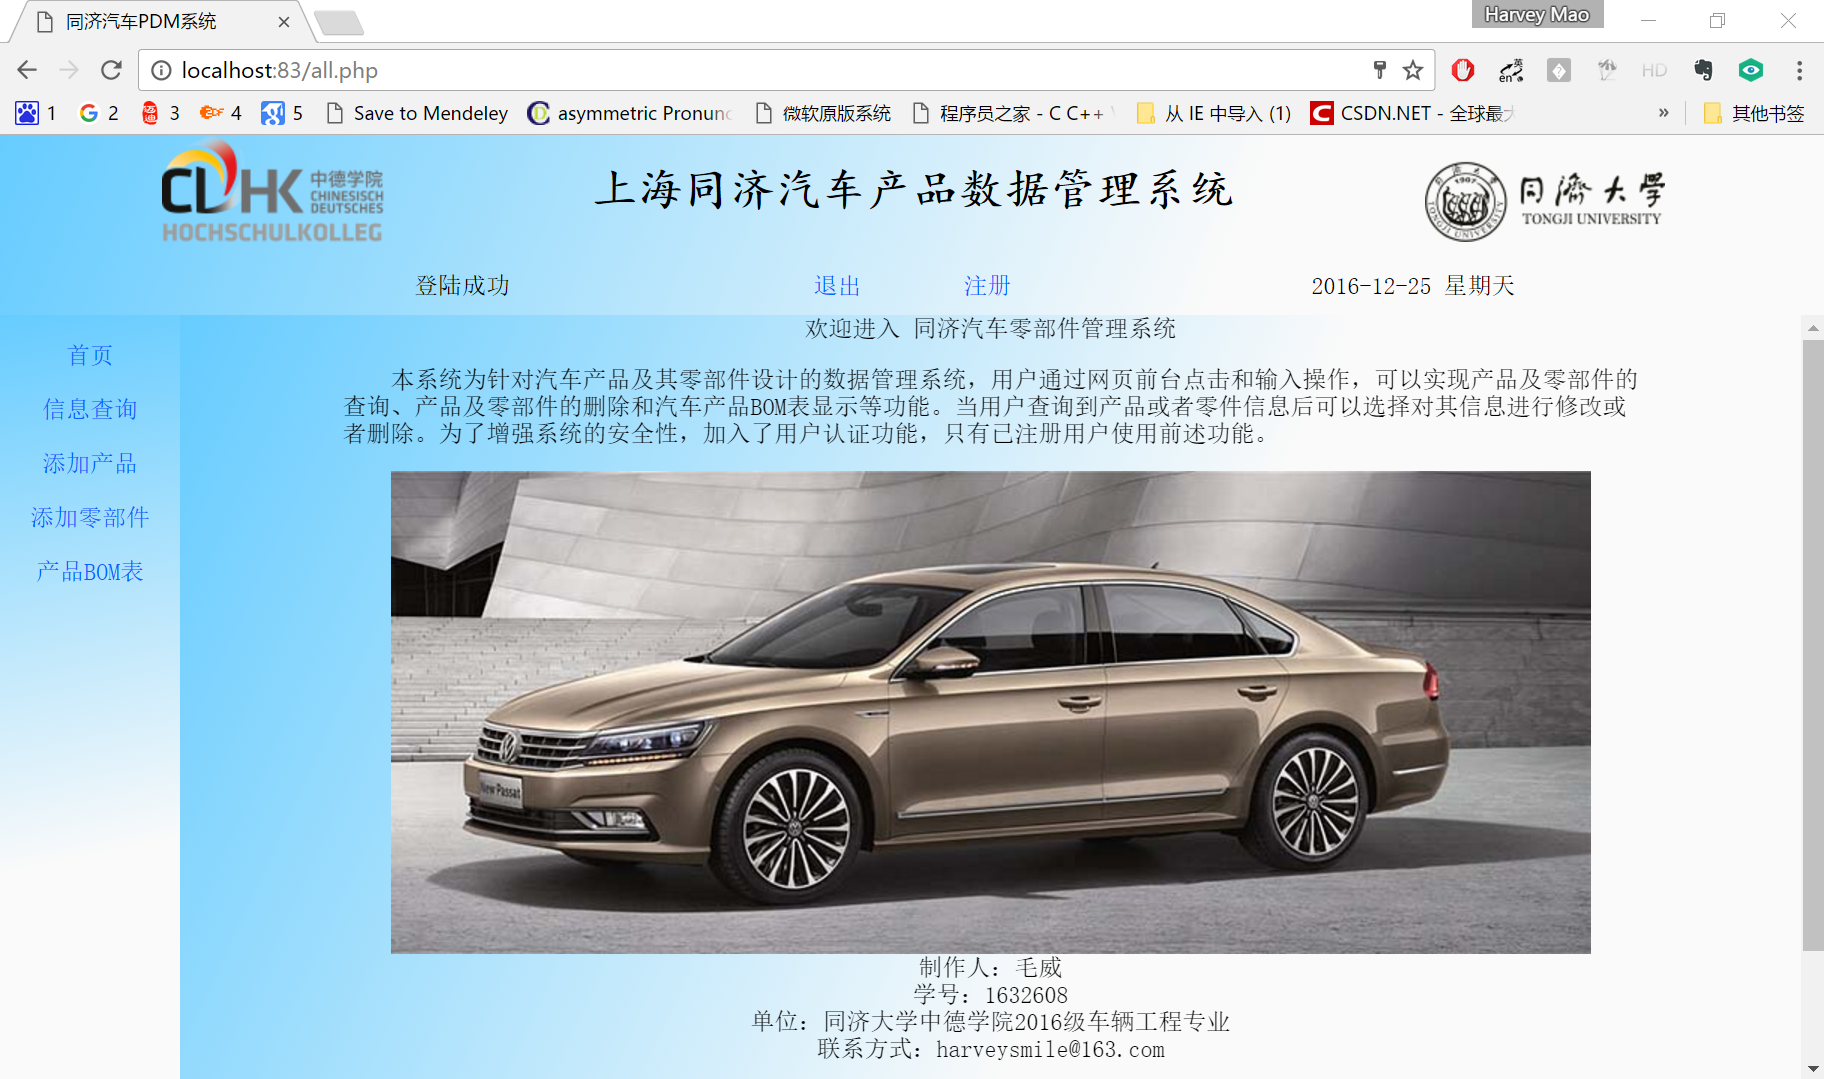
\includegraphics[width=0.9\linewidth]{figure/index}
\caption{汽车PDM主界面}
\label{fig:index1}
\end{figure}

\subsection{用户认证}
增加对用户的身份认证可以提高数据的安全性。非注册用户无法访问数据库完成各项功能。

在未登录网页的情况下点击主页\underline{信息查询、添加产品、添加零部件和产品BOM表},将弹出未登录对话框,如图\ref{fig:nologin}。
\begin{figure}[H]
\centering
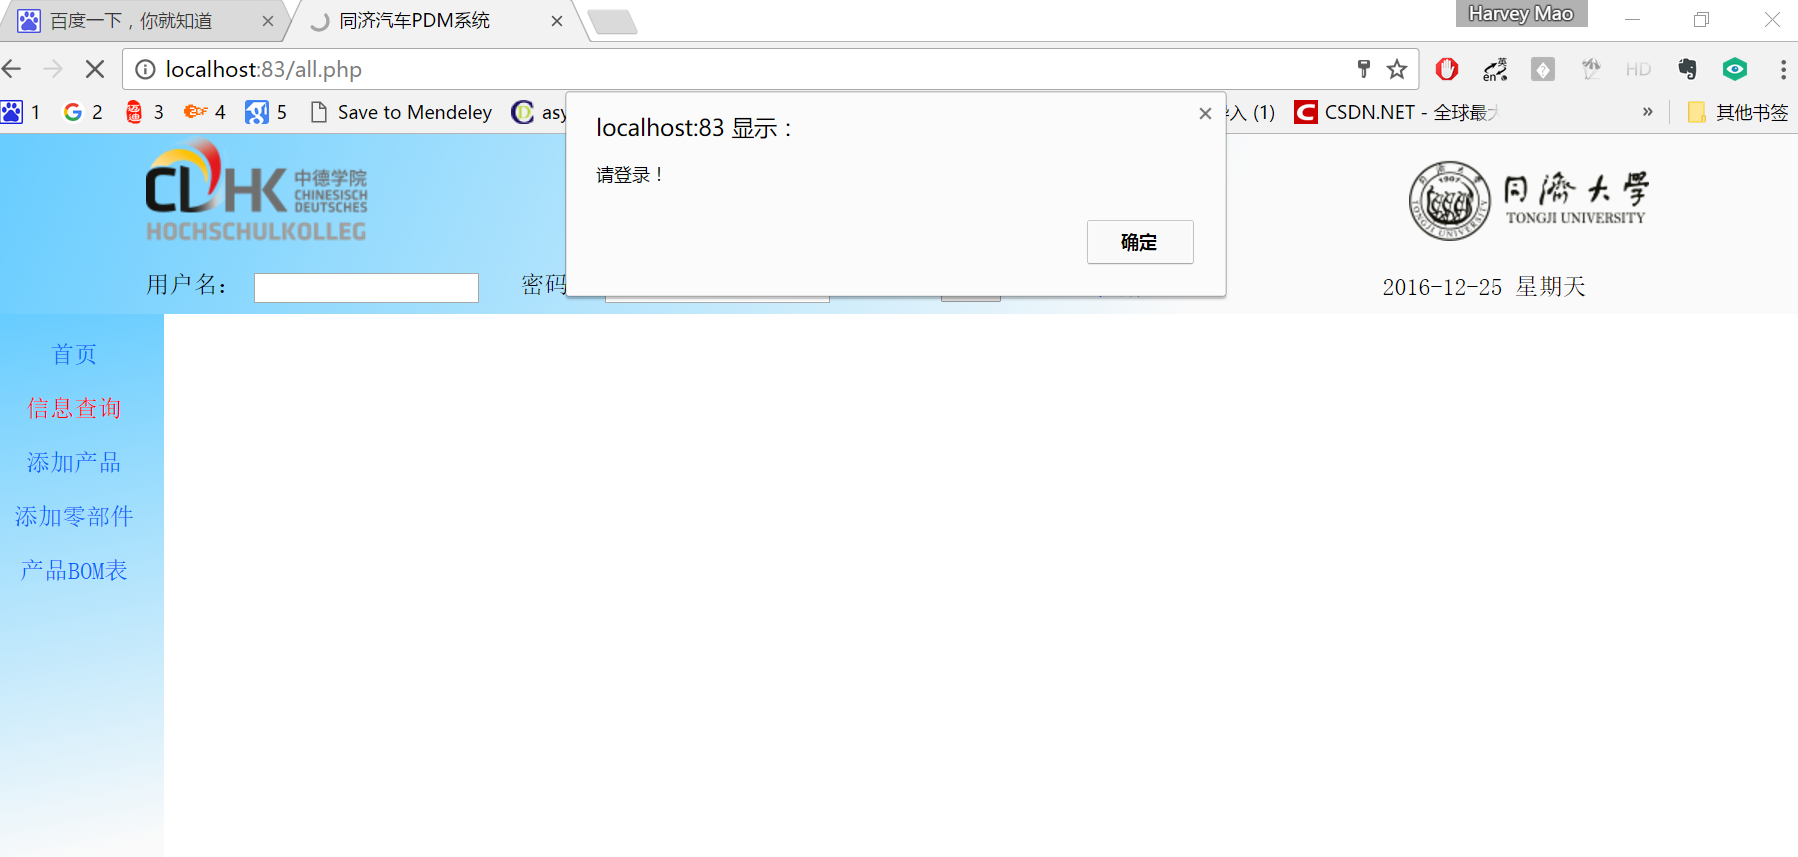
\includegraphics[width=0.9\linewidth]{figure/nologin}
\caption{未登录提醒}
\label{fig:nologin}
\end{figure}

点击\underline{注册},如图\ref{fig:reg}所示,输入用户名和密码,注意2次输入密码一致,否则注册失败。
\begin{figure}[H]
\centering
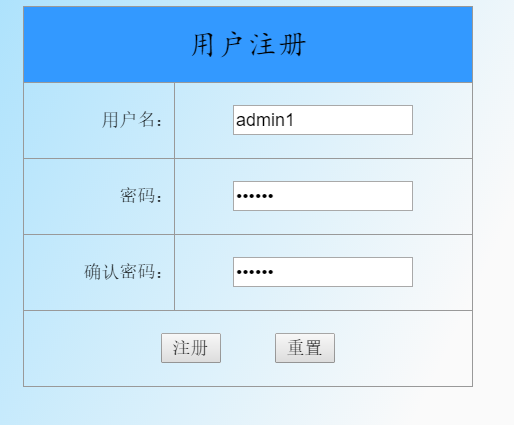
\includegraphics[width=0.8\linewidth]{figure/reg}
\caption{注册}
\label{fig:reg}
\end{figure}

输入用户名和密码,点击\underline{登陆},如图\ref{fig:printlogin}所示。
\begin{figure}[H]
\centering
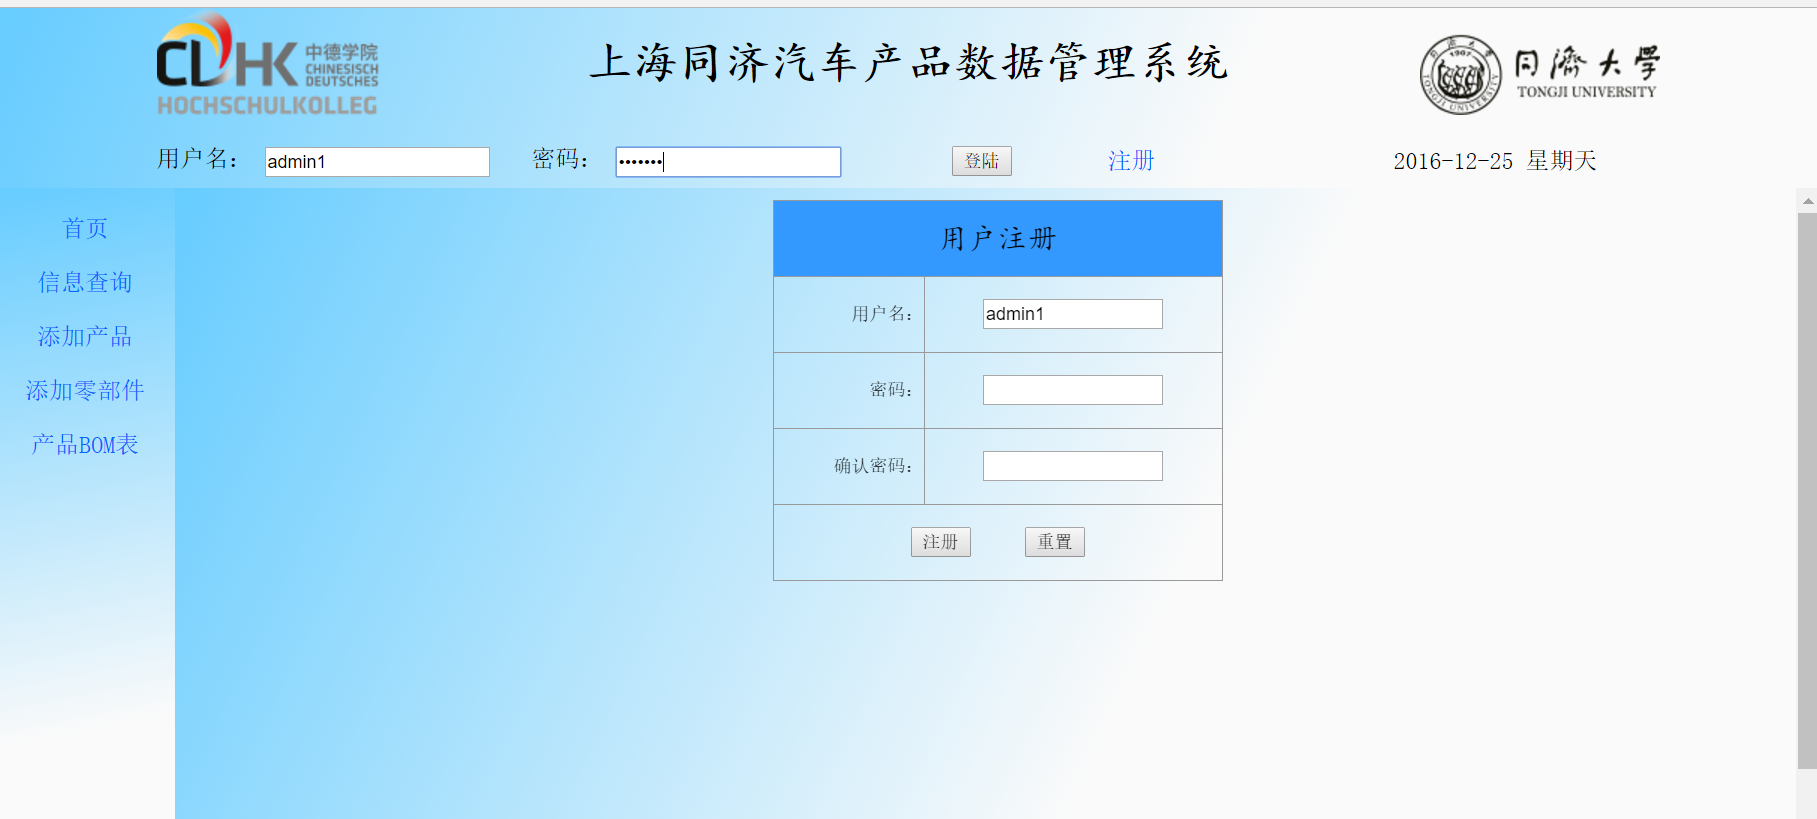
\includegraphics[width=0.7\linewidth]{figure/printlogin}
\caption{登陆}
\label{fig:printlogin}
\end{figure}

如果用户名和密码输入正确,则显示登陆成功,如图\ref{fig:sucesslogin}所示,否则登陆失败,如图\ref{fig:loslogin}所示.
\begin{figure}[H]
\centering
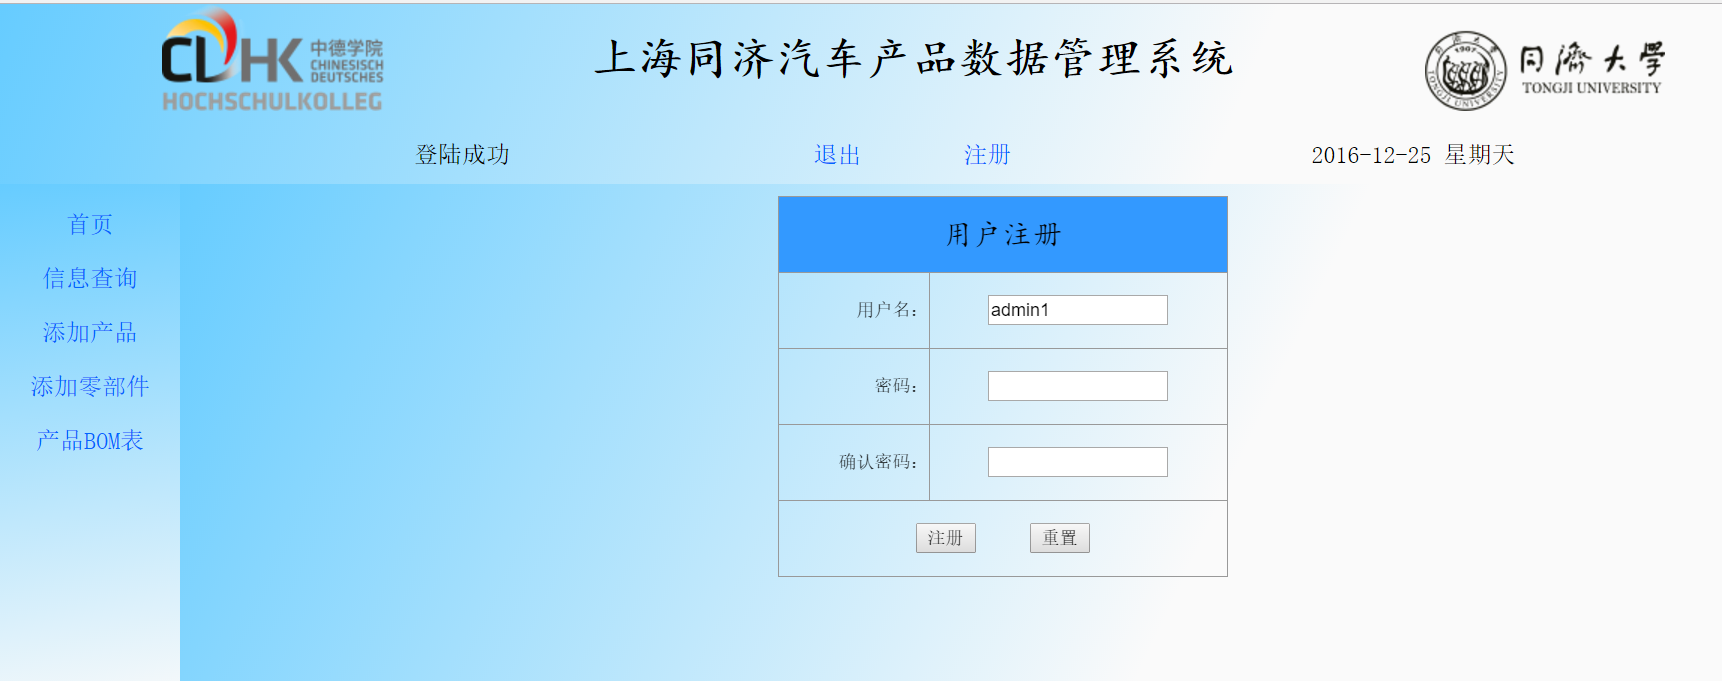
\includegraphics[width=0.9\linewidth]{figure/sucesslogin}
\caption{登陆成功}
\label{fig:sucesslogin}
\end{figure}

\begin{figure}[H]
\centering
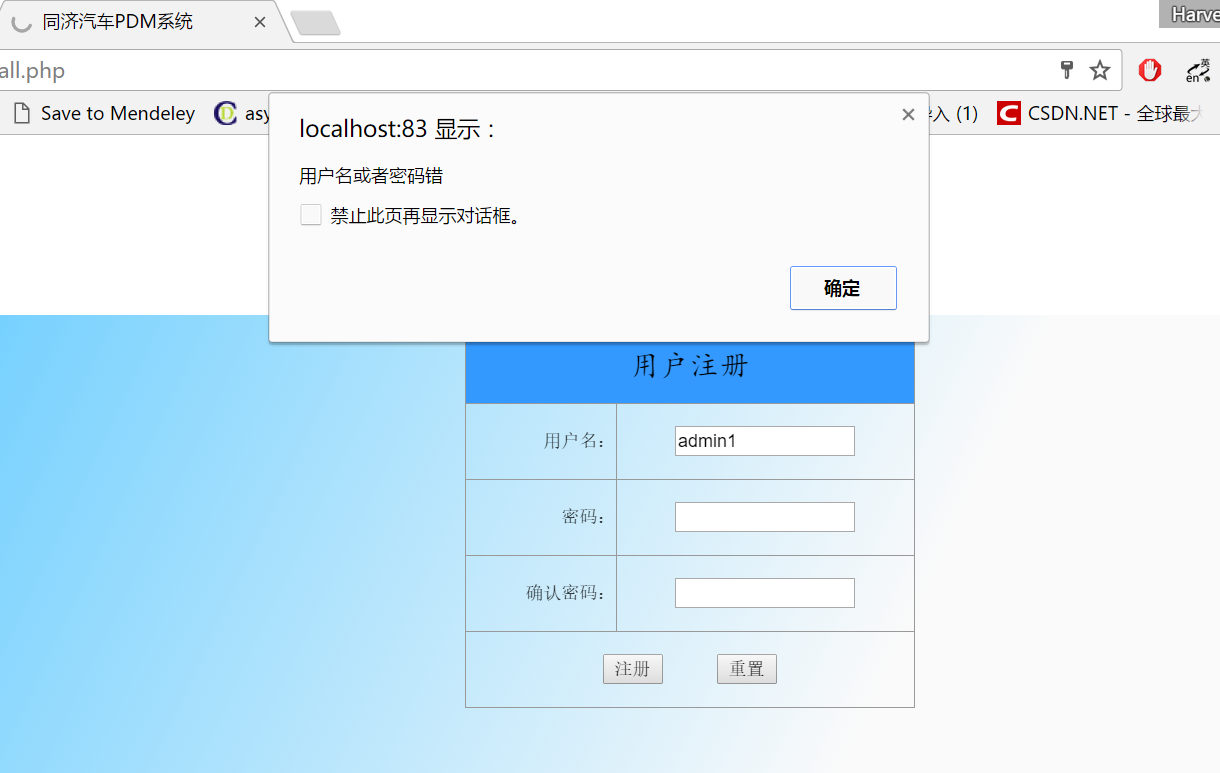
\includegraphics[width=0.9\linewidth]{figure/loslogin}
\caption{登陆失败弹框}
\label{fig:loslogin}
\end{figure}



\subsection{记录查询}

\subsubsection{简单查询模式}
点击主页\underline{信息查询},进入记录查询查询页面,如图\ref{fig:simplesearch}所示。简单查询模式支持某一字段(型号、名词、编号、制造商、产地)和价格做为查询条件,其中价格项目2个输入框分别为价格的最小最大值。三个输入框可以只输入1个或者输入2个或者全部输入,输入值之间构成``与''逻辑。
\begin{figure}[H]
\centering
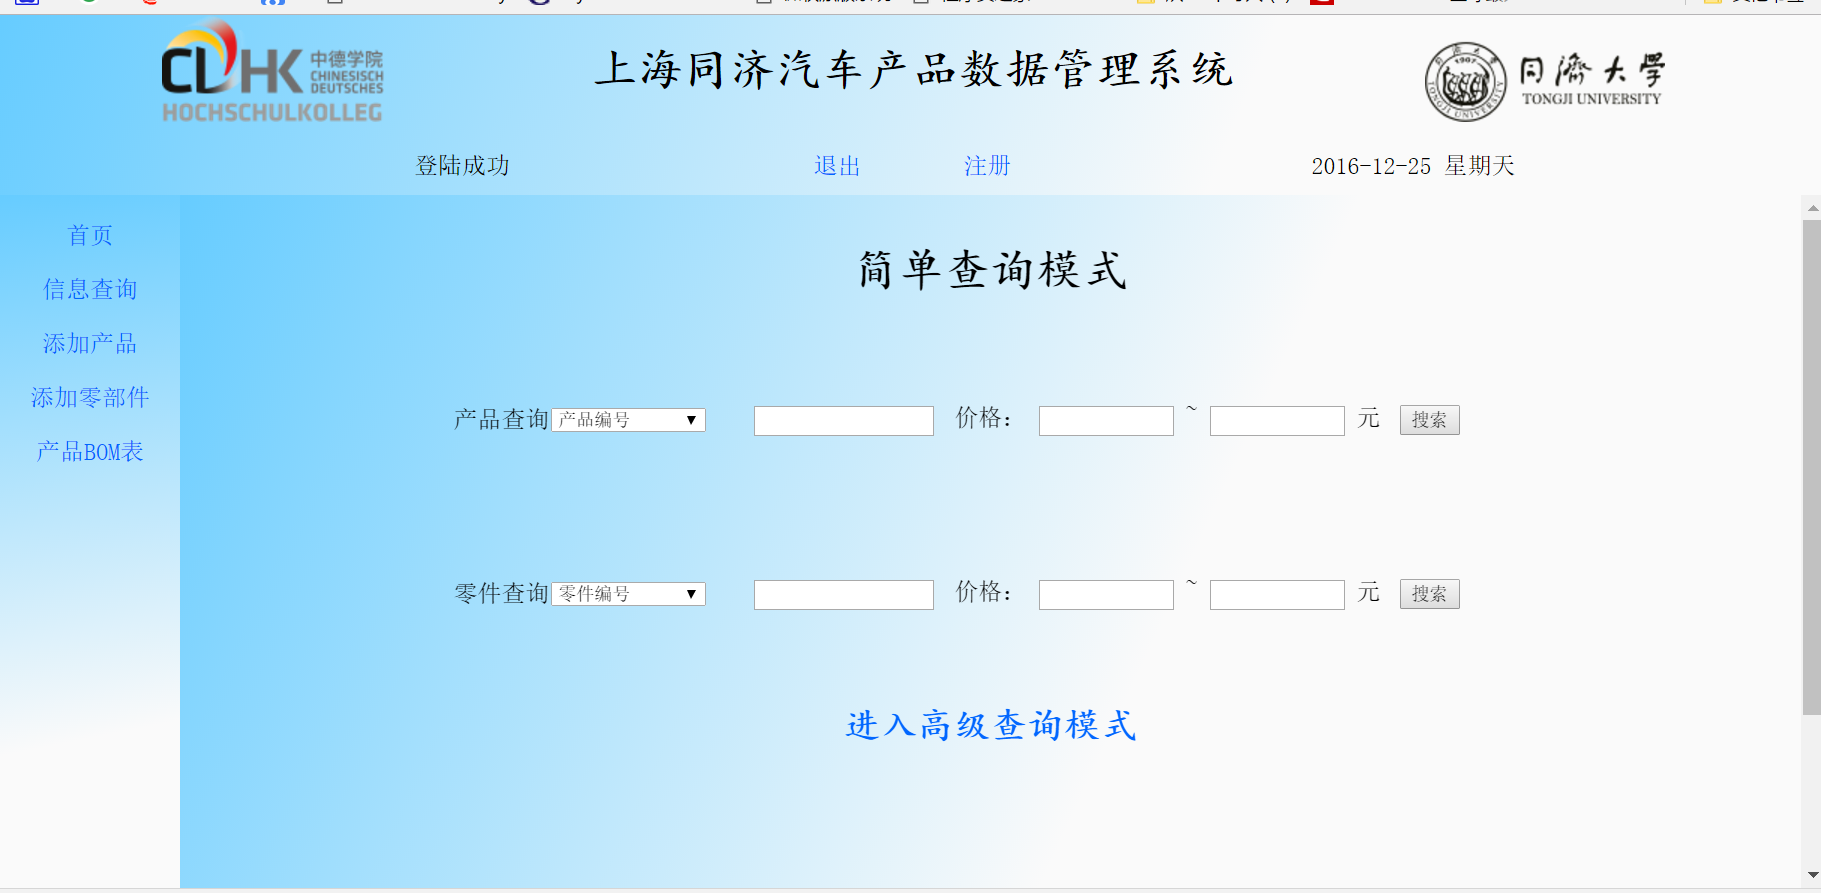
\includegraphics[width=0.8\linewidth]{figure/simplesearch}
\caption{信息查询页面}
\label{fig:simplesearch}
\end{figure}

在产品查询简单查询模式中输入如图\ref{fig:spsearch_prd_name}所示的条件,即查询产品名称为POLO的汽车产品,点击\underline{搜索},查询结果如图\ref{fig:spsearch_prd_name_result}所示。
\begin{figure}[H]
\centering
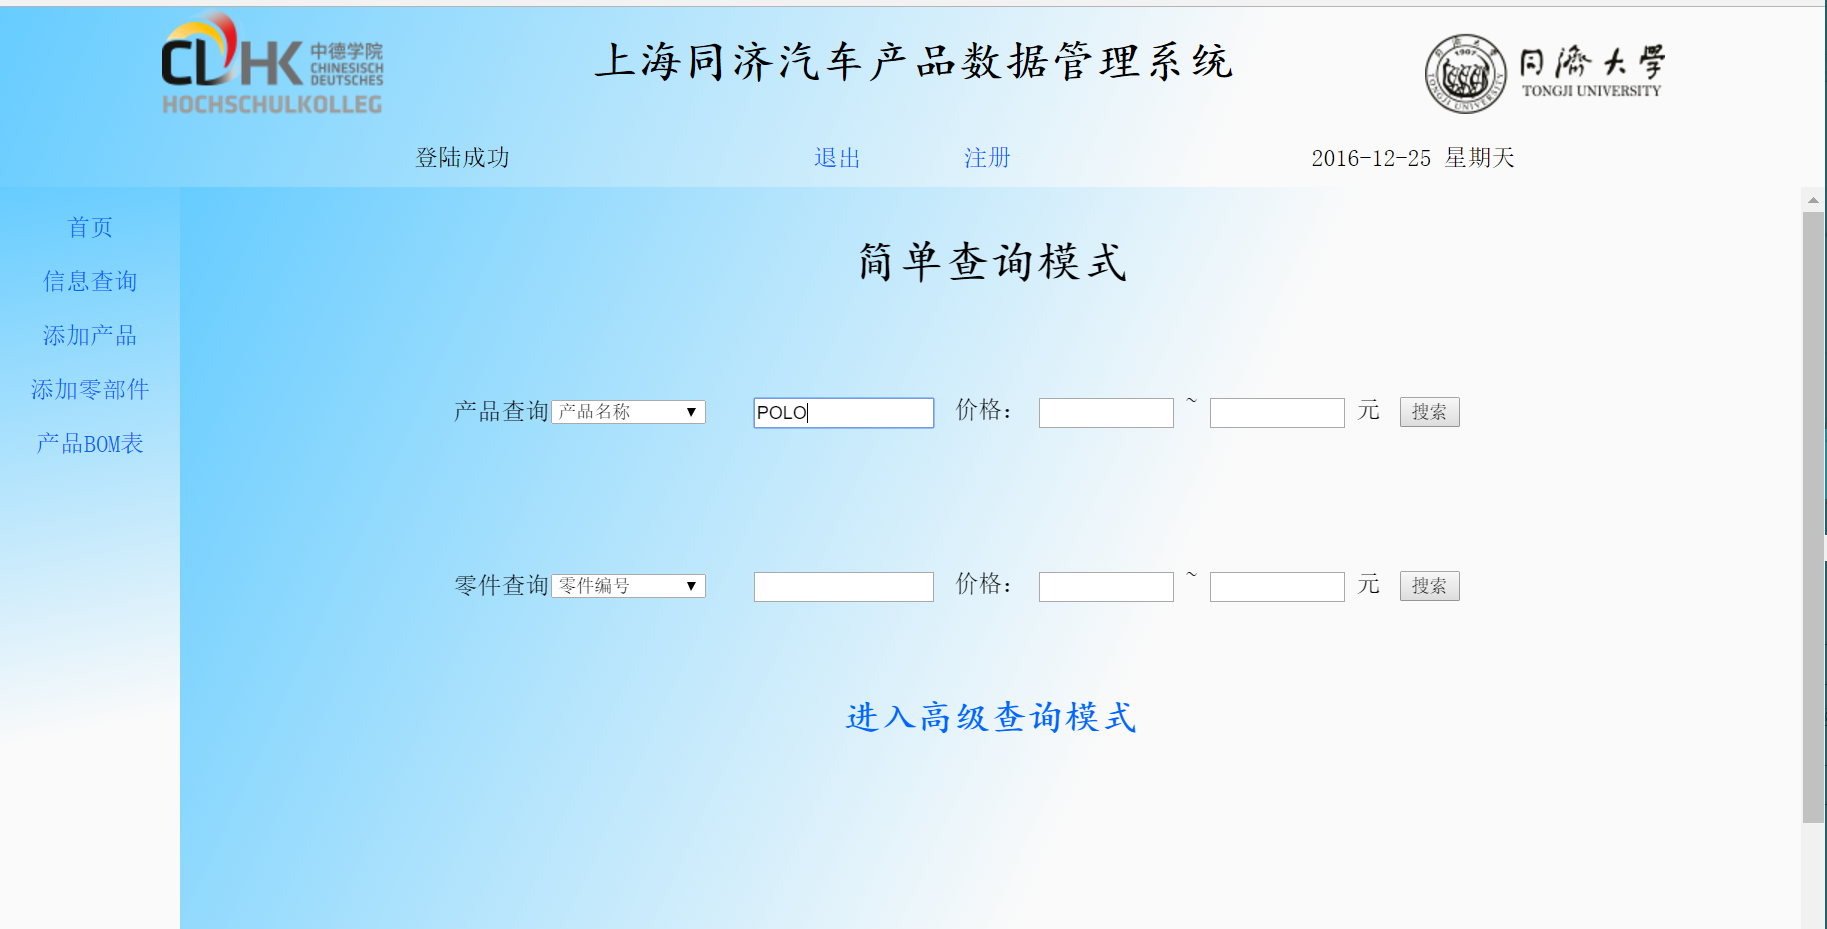
\includegraphics[width=0.9\linewidth]{figure/spsearch_prd_name}
\caption{简单搜索-产品名称}
\label{fig:spsearch_prd_name}
\end{figure}
\begin{figure}[H]
\centering
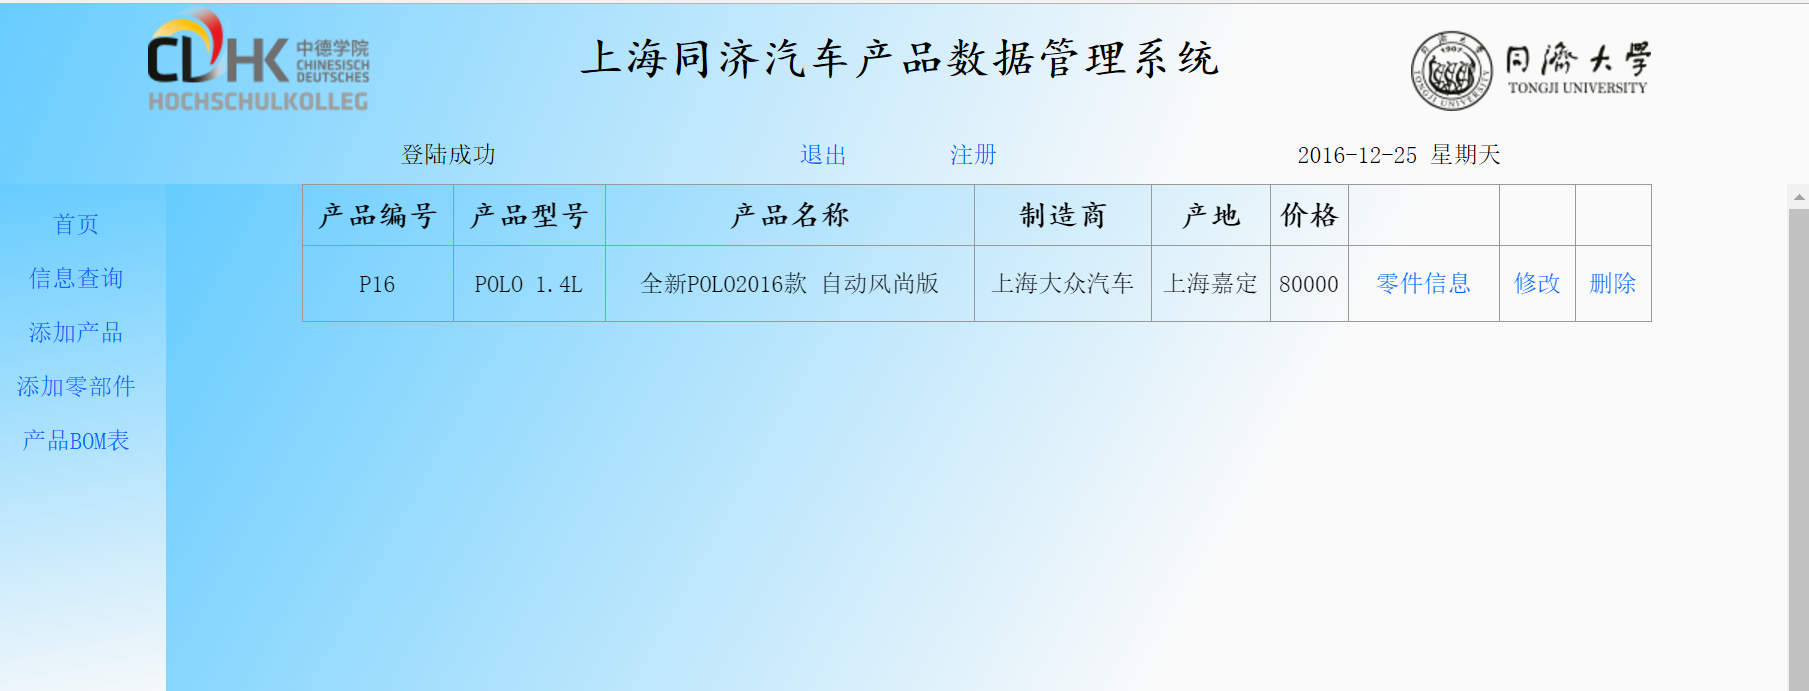
\includegraphics[width=0.9\linewidth]{figure/spsearch_prd_name_result}
\caption{简单搜索-产品名称-查询结果}
\label{fig:spsearch_prd_name_result}
\end{figure}

在零件查询简单查询模式中输入如图\ref{fig:spsea_part_area_price}所示的条件,即查询零件产地为上海并且价格低于1000元的汽车零件,点击\underline{搜索},查询结果如图\ref{fig:spsea_part_area_price_result}所示。
\begin{figure}[H]
\centering
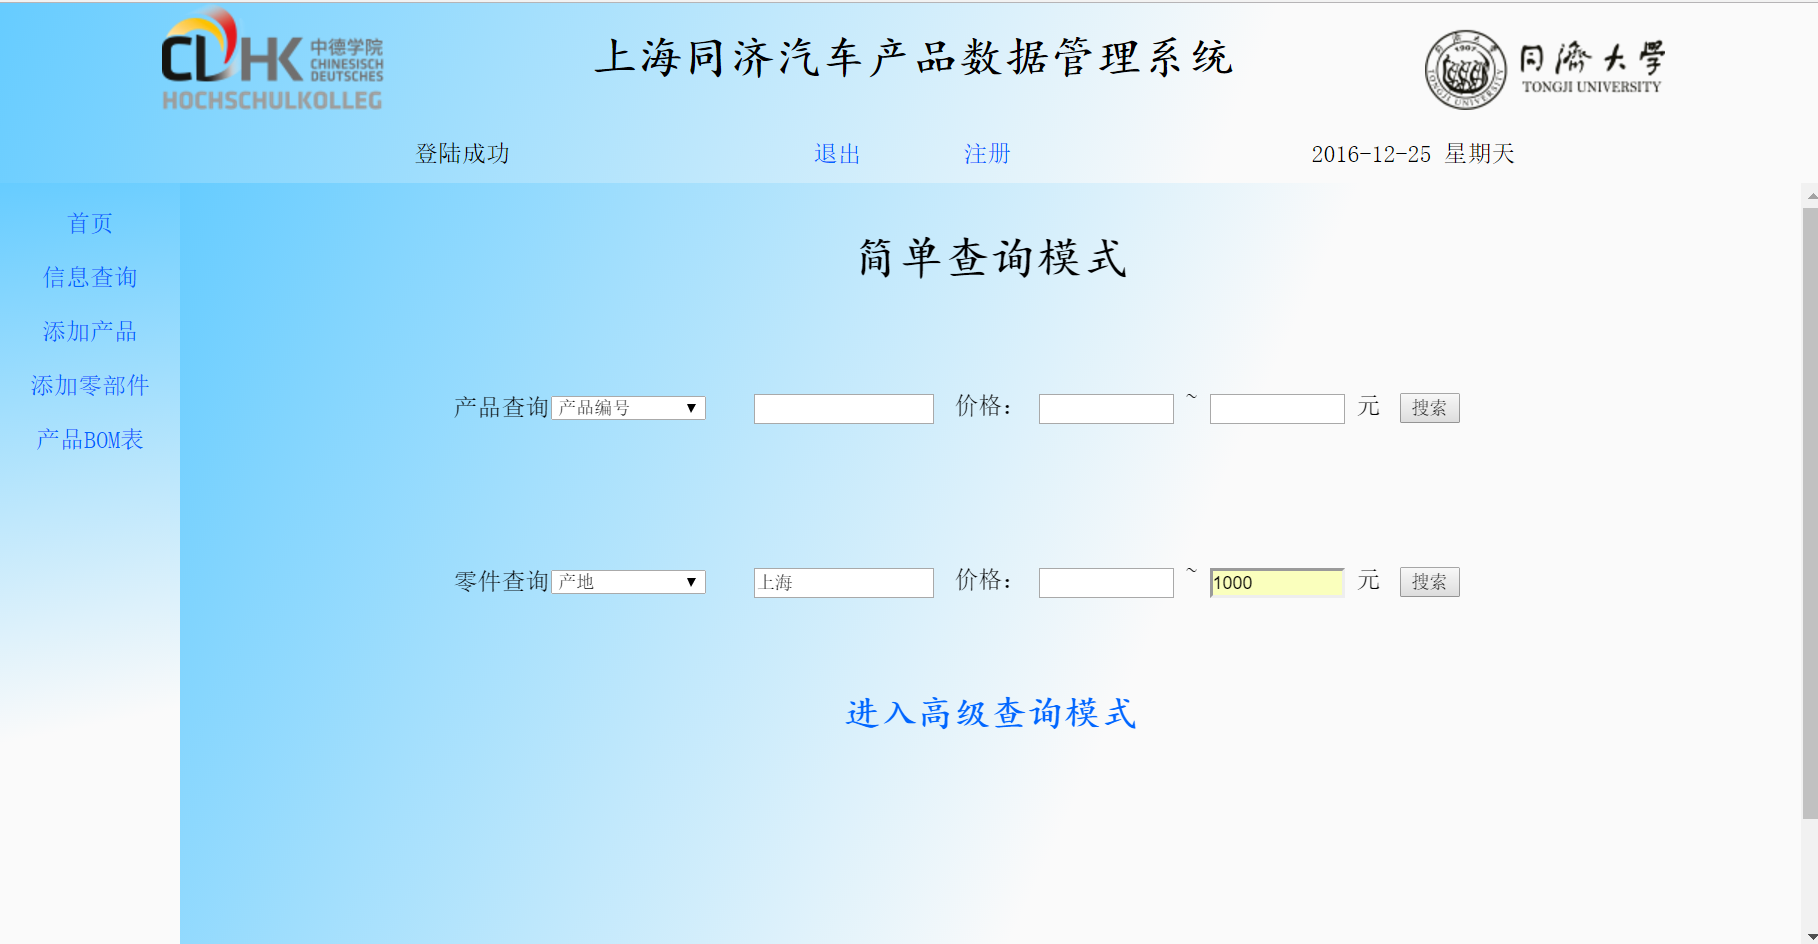
\includegraphics[width=0.9\linewidth]{figure/spsea_part_area_price}
\caption{简单查询-零件查询-产地/价格}
\label{fig:spsea_part_area_price}
\end{figure}

\begin{figure}[H]
\centering
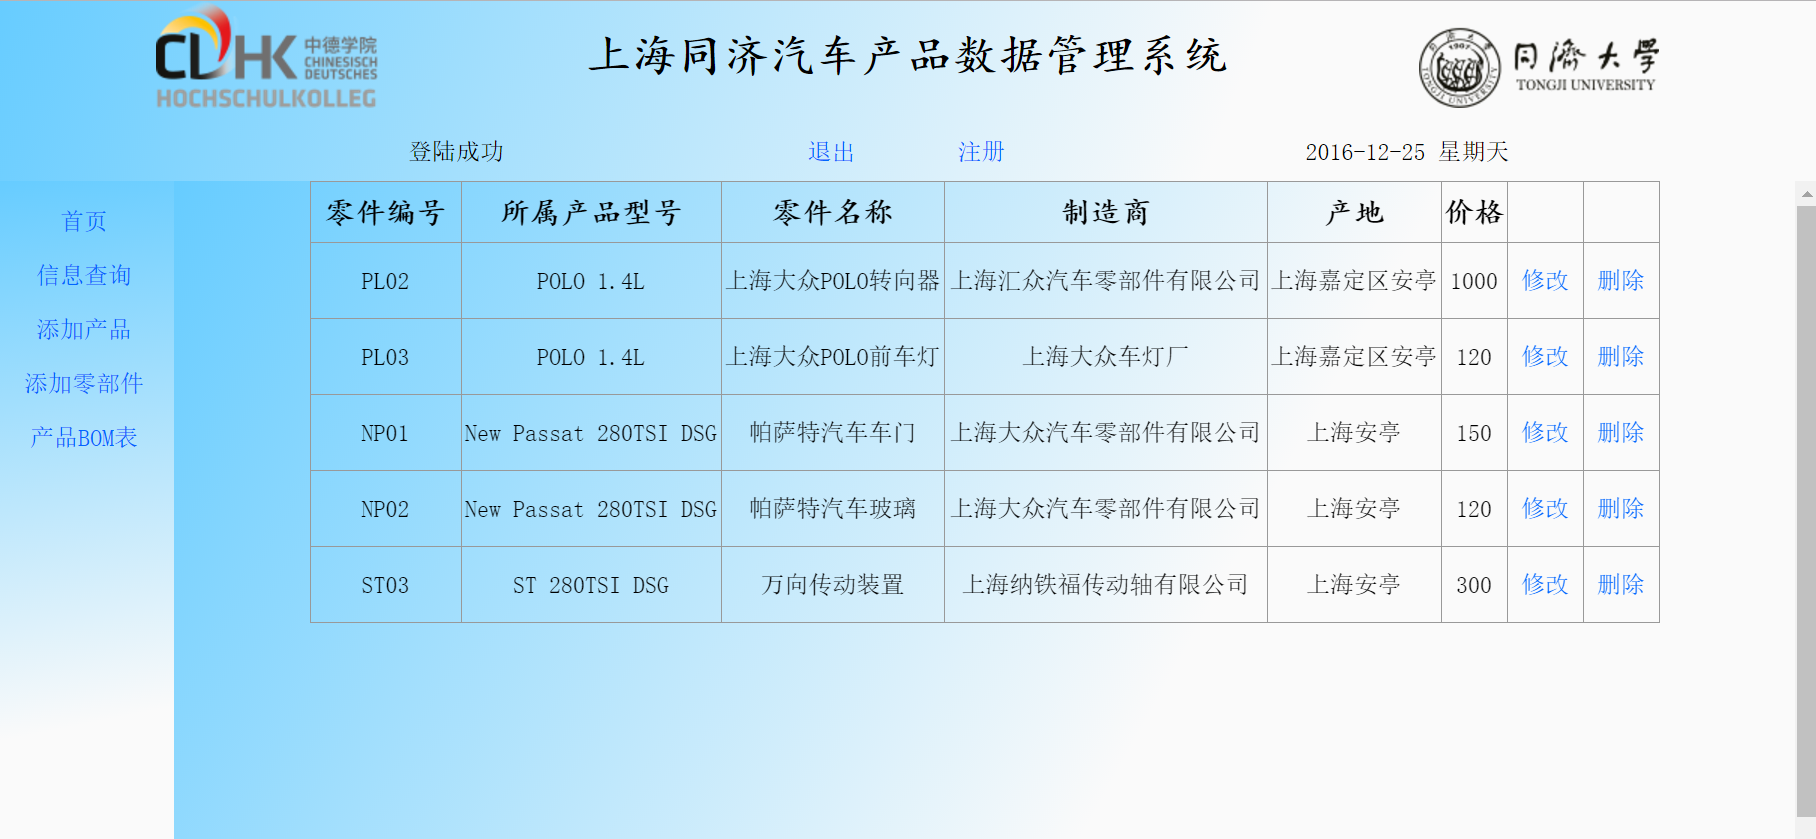
\includegraphics[width=0.9\linewidth]{figure/spsea_part_area_price_result}
\caption{简单查询-零件查询-产地/价格-查询结果}
\label{fig:spsea_part_area_price_result}
\end{figure}

本文设计的查询系统中各个文本字段值均采用模糊匹配方法,如图\ref{fig:spsea_part_area_price_result}所示,只要产地中包含图\ref{fig:spsea_part_area_price}中产地值\textbf{上海}的记录都视为满足条件。

对于价格字段中的输入框,如果只给左边框赋值$L$,则表示条件:价格$\ge L$。,如果只给右边框赋值$R$,则表示条件:价格$\le R$。如果左框赋值$L$,右框赋值$R$,则表示条件:$L \le$价格$\le R$。

如果输入的价格不为数字(如图\ref{fig:price_error}),则系统会弹出``价格必须为数字''的提示框(如图\ref{fig:price_error_alert})。
\begin{figure}[H]
\centering
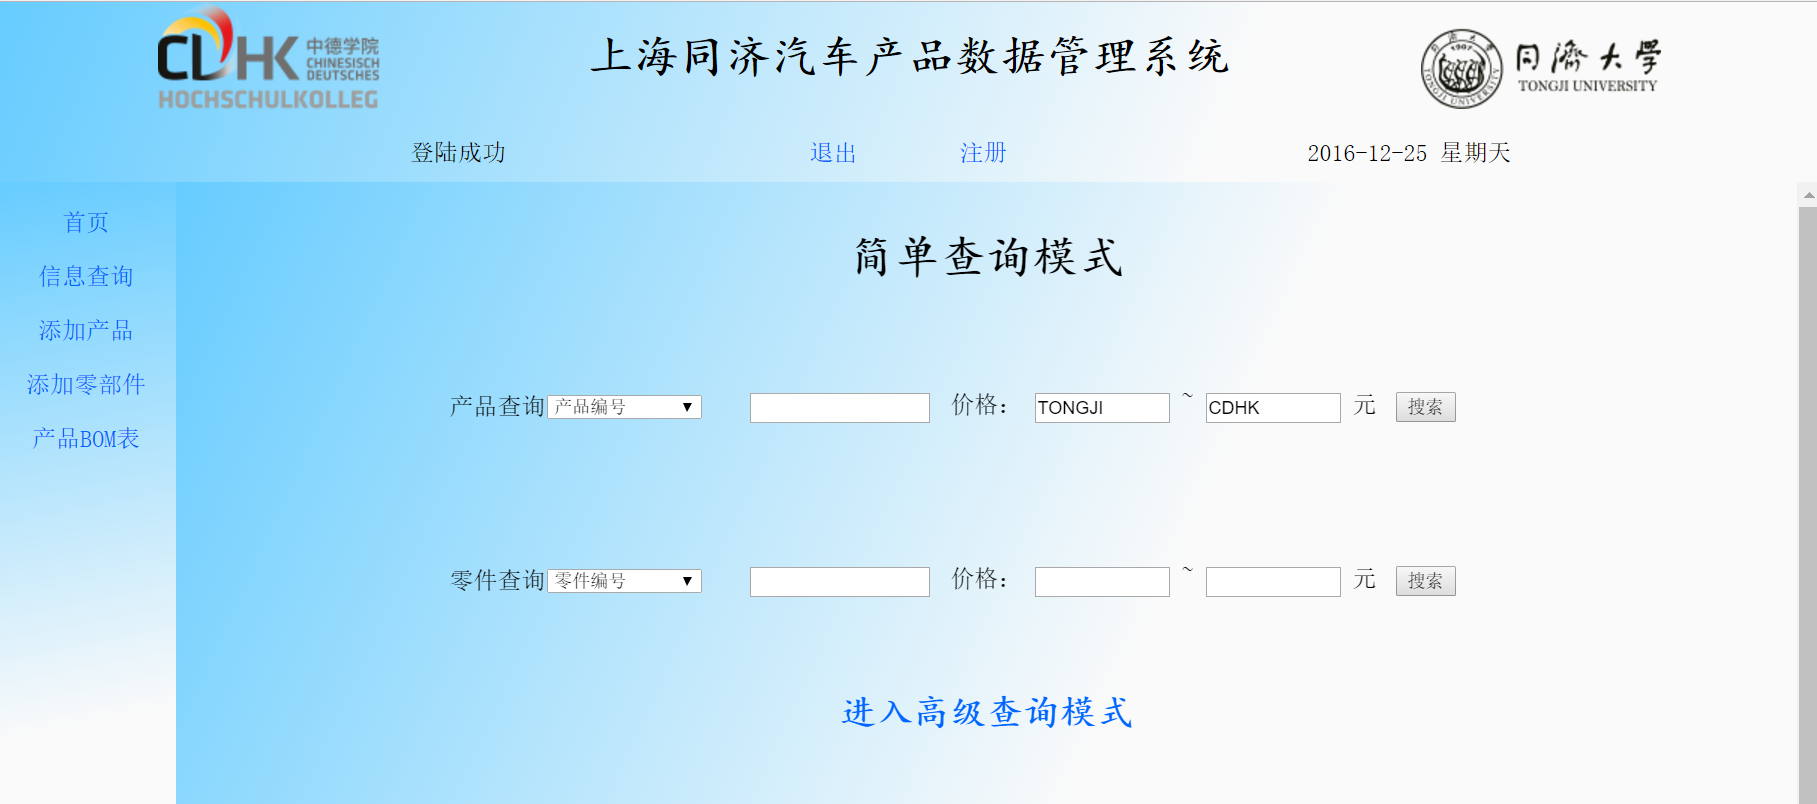
\includegraphics[width=0.9\linewidth]{figure/price_error}
\caption{错误价格格式}
\label{fig:price_error}
\end{figure}
\begin{figure}[H]
\centering
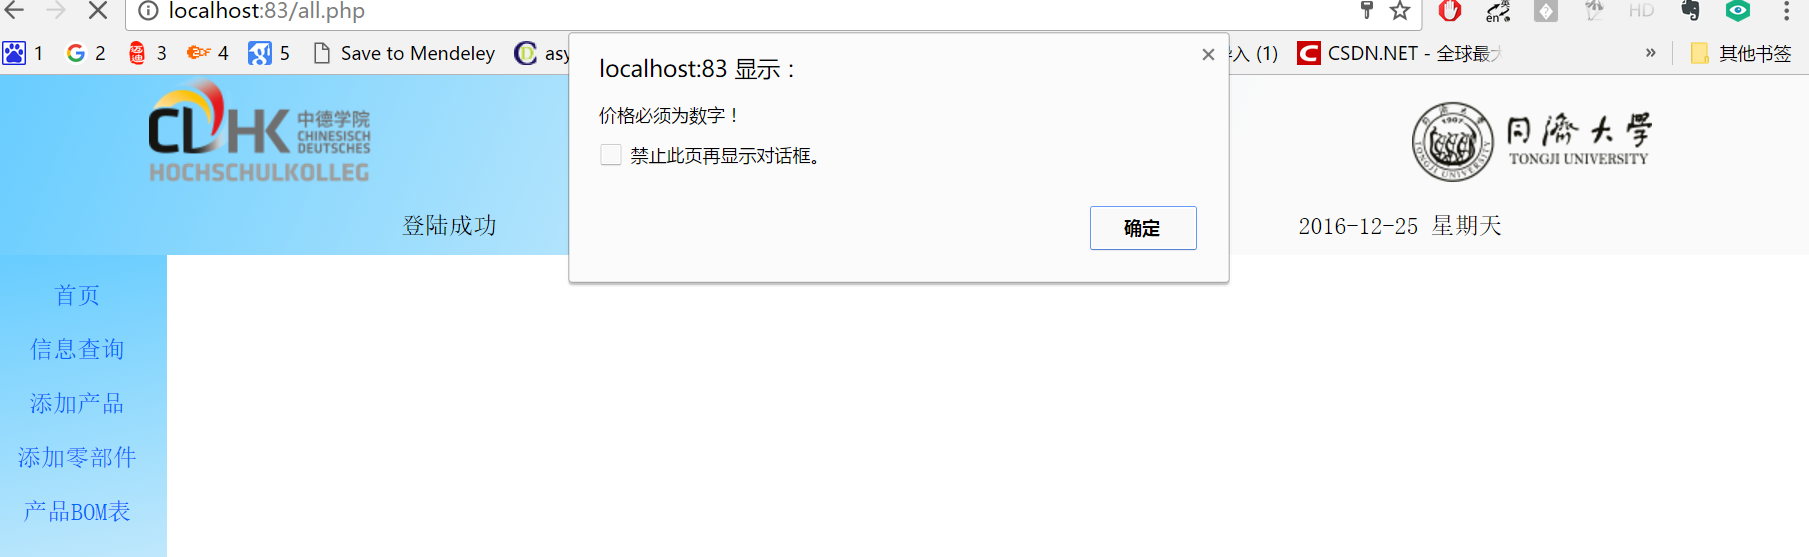
\includegraphics[width=0.9\linewidth]{figure/price_error_alert}
\caption{价格错误弹框}
\label{fig:price_error_alert}
\end{figure}

如果没有符合条件(如图\ref{fig:noreulscond})的结果,则系统会弹出``没有符合条件的记录''提示框(如图\ref{fig:noresult})。
\begin{figure}[H]
\centering
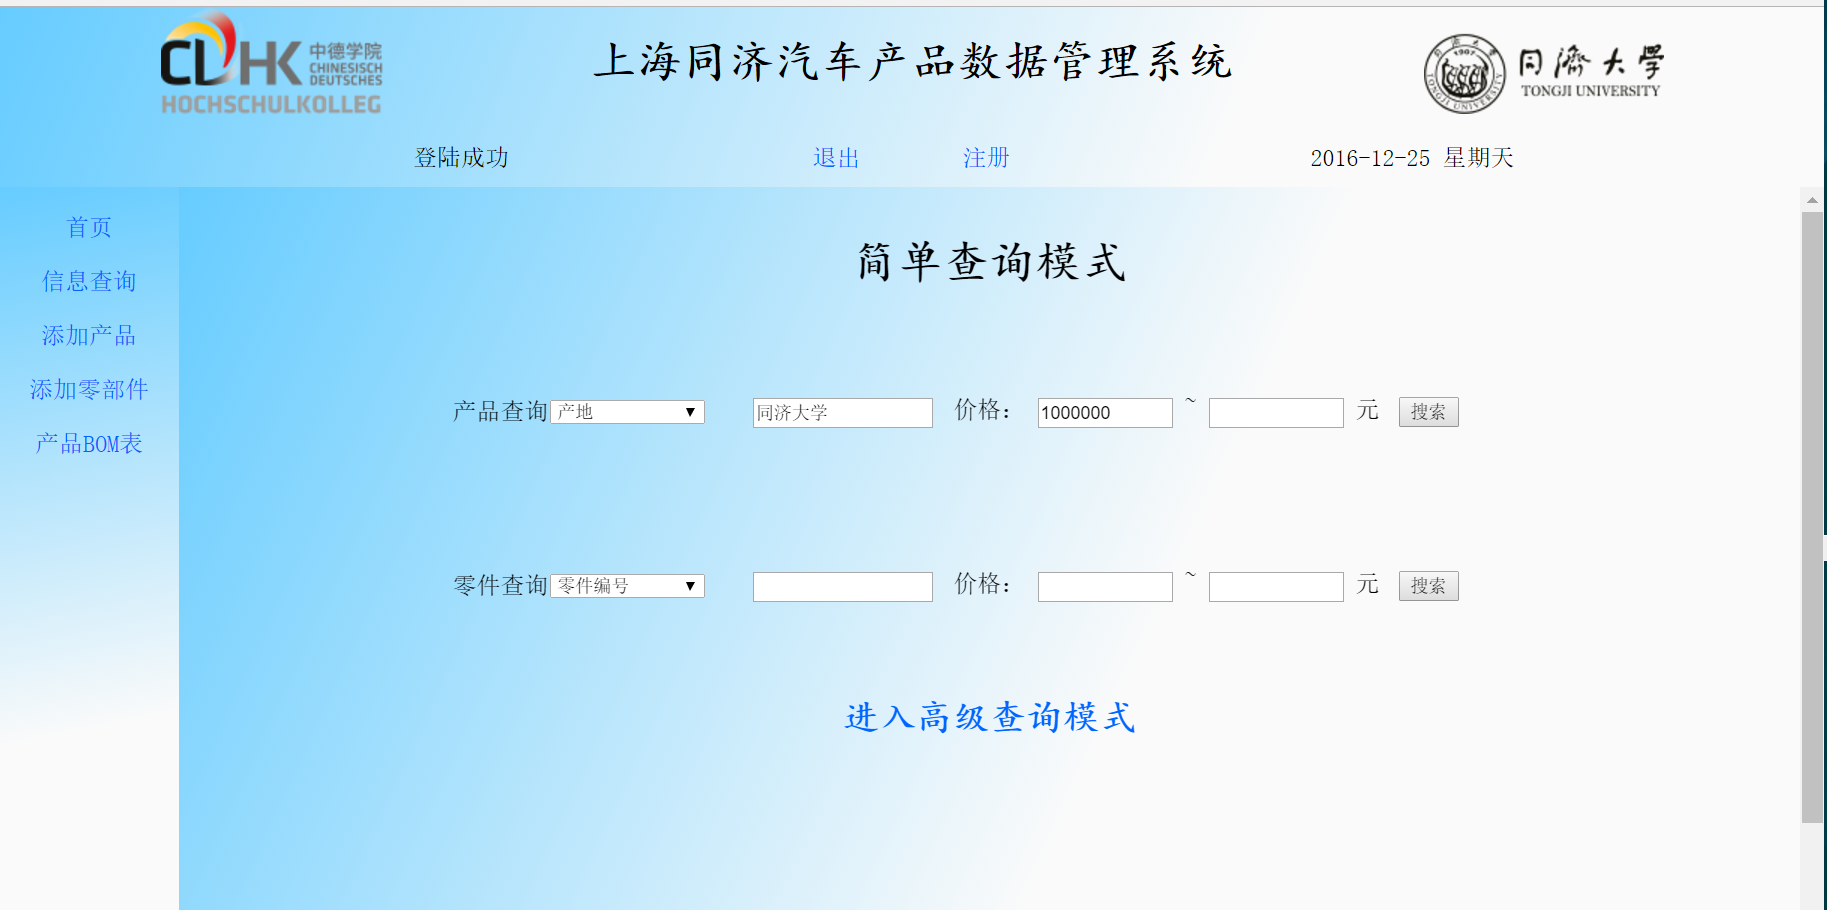
\includegraphics[width=0.9\linewidth]{figure/noreulscond}
\caption{无记录条件}
\label{fig:noreulscond}
\end{figure}

\begin{figure}[H]
\centering
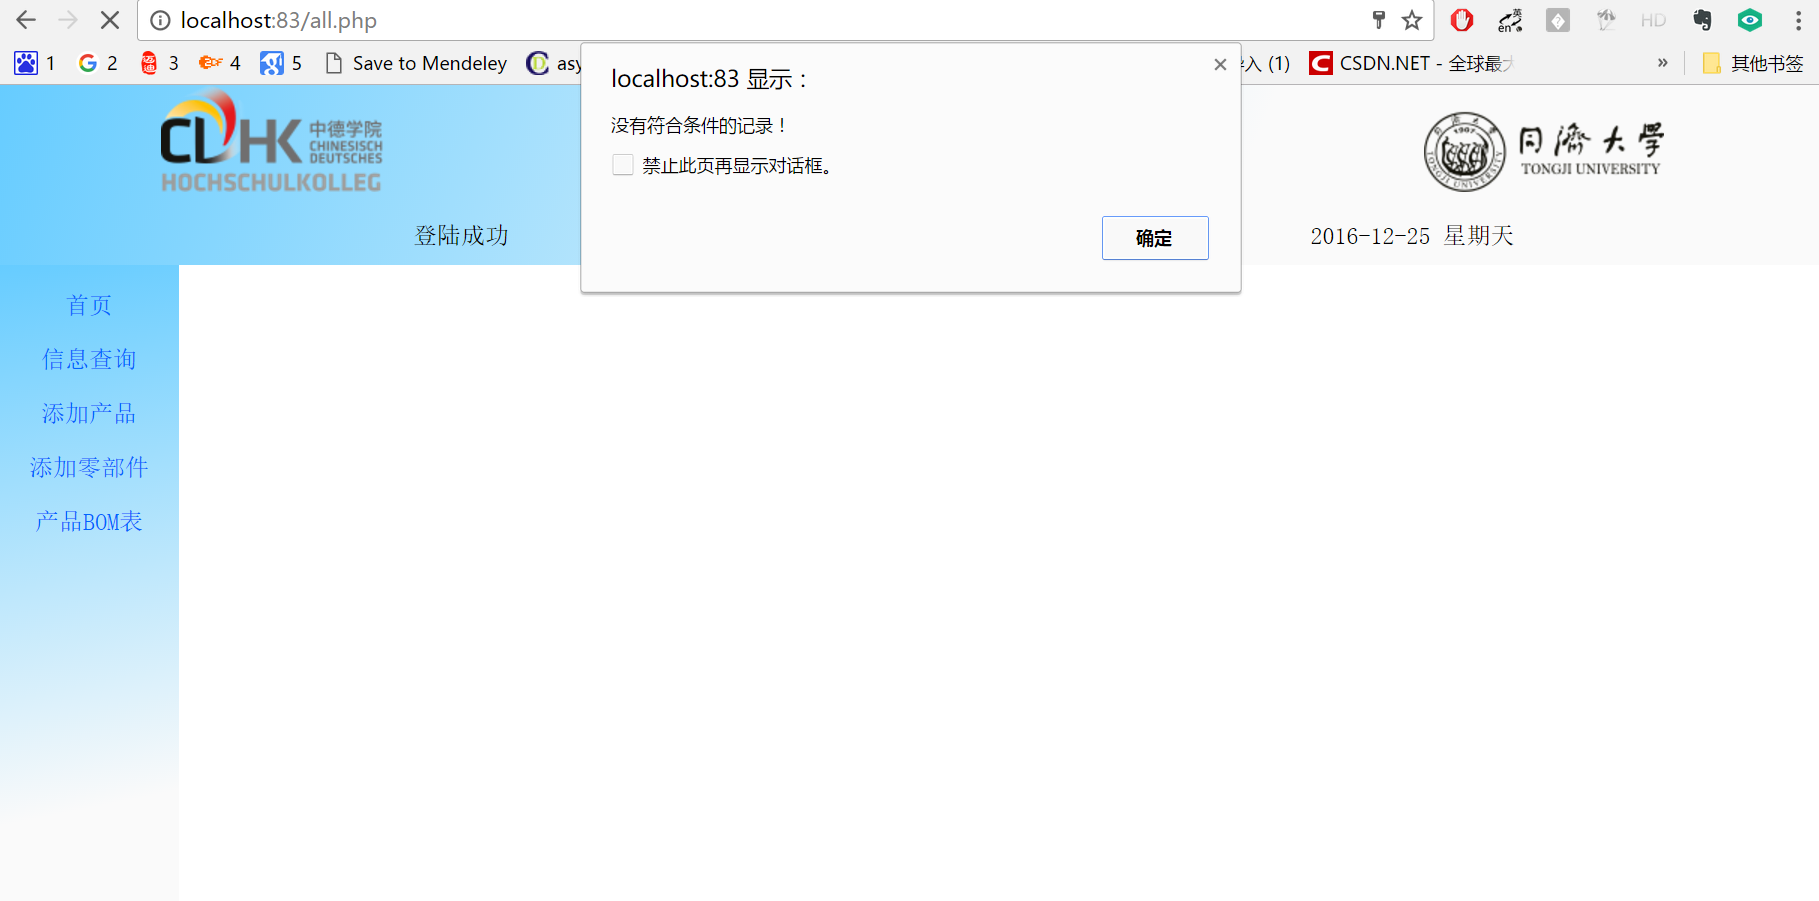
\includegraphics[width=0.9\linewidth]{figure/noresult}
\caption{``无符合条件记录''弹框}
\label{fig:noresult}
\end{figure}

\subsubsection{高级查询模式}
依次点击\underline{信息查询}$\to $\underline{进入高级查询模式}(如图\ref{fig:seniorSearInto_PxCook}),即可进入高级查询界面(如图\ref{fig:seniorSear})。
\begin{figure}[H]
\centering
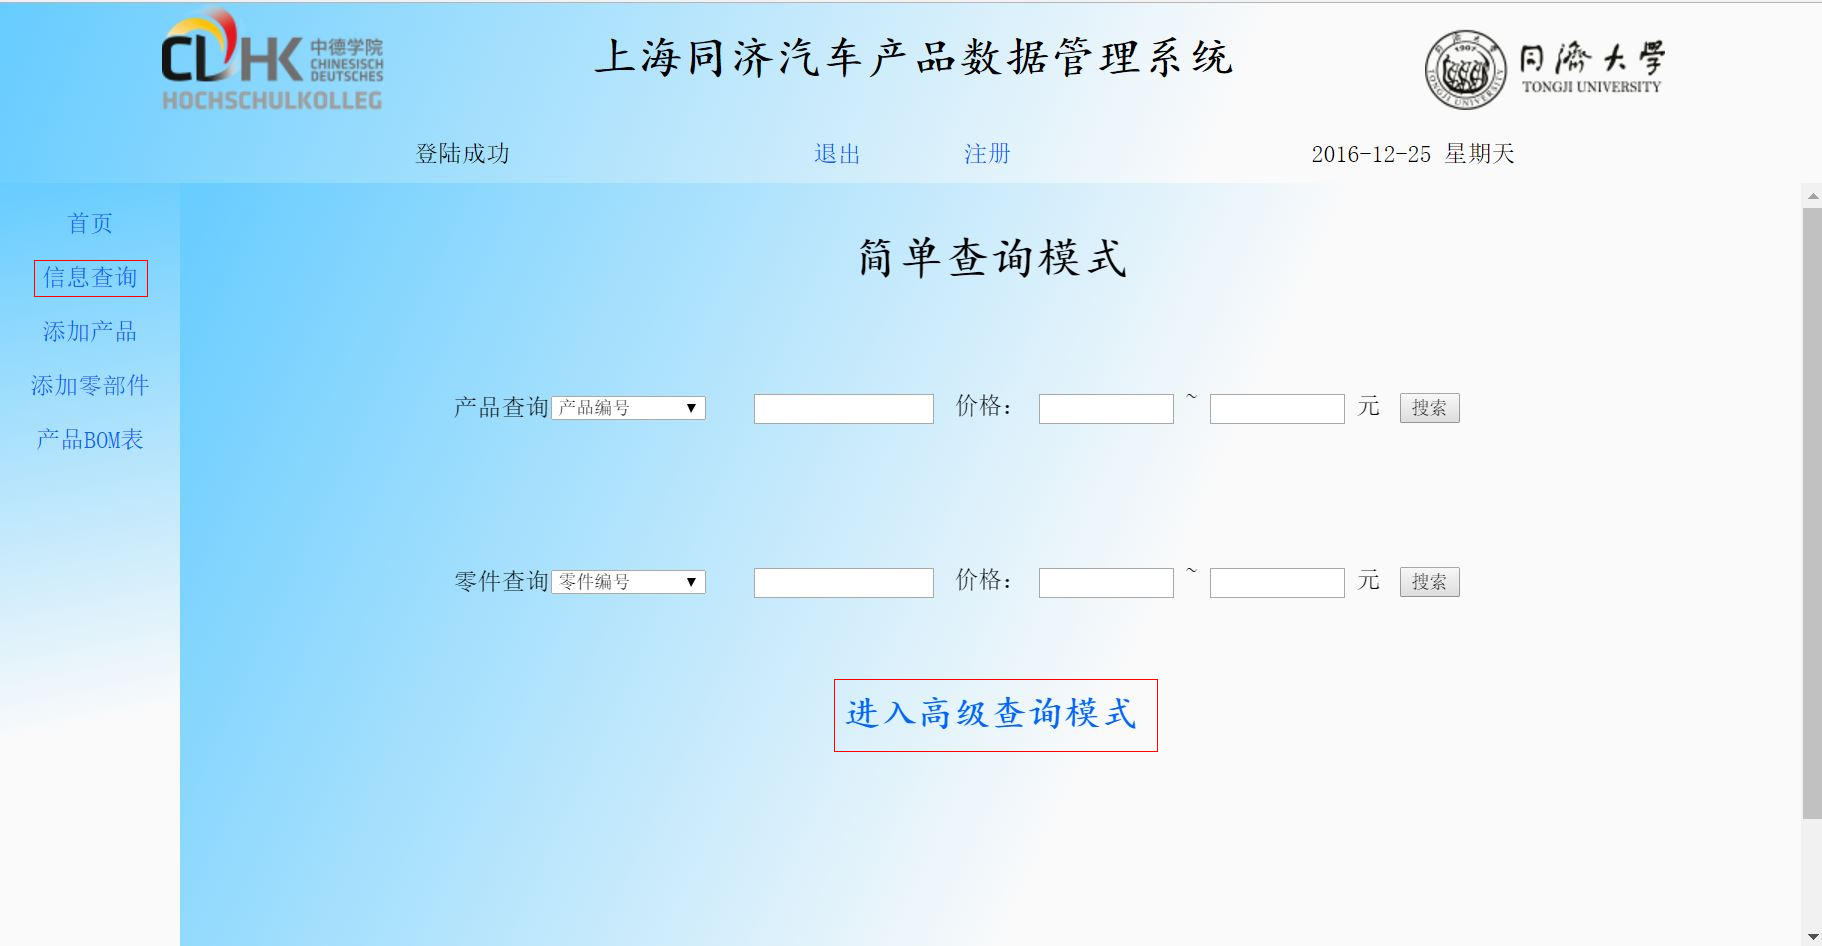
\includegraphics[width=0.9\linewidth]{figure/seniorSearInto_PxCook}
\caption{进入高级查询模式}
\label{fig:seniorSearInto_PxCook}
\end{figure}

\begin{figure}[H]
\centering
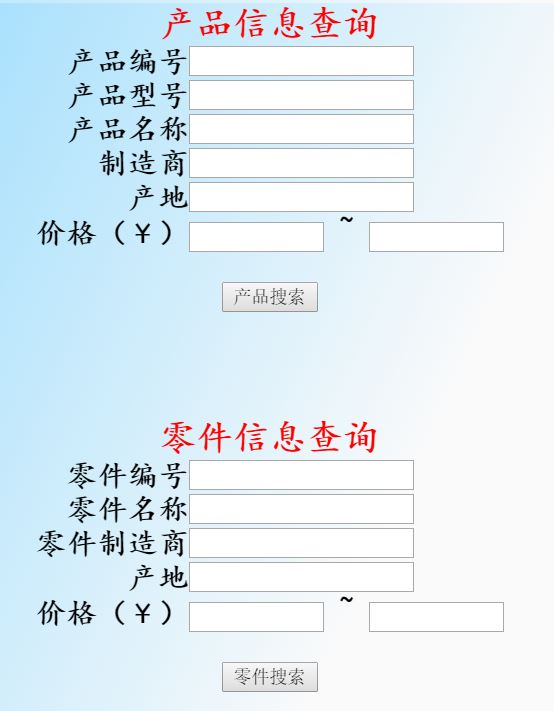
\includegraphics[width=0.7\linewidth]{figure/seniorSear}
\caption{高级查询模式}
\label{fig:seniorSear}
\end{figure}

高级查询模式支持所有字段任意组合成``与''逻辑的查询,可以给所有字段赋值,也可以只给部分字段赋值。

例如,在高级查询模式下,搜索条件如图\ref{fig:seniorPartSea}所示,即条件为产地含``武汉''字样、公司含``东风''字样、价格不超过200元,搜索结果如图\ref{fig:seniorPartRes}所示。

\begin{figure}[H]
\centering
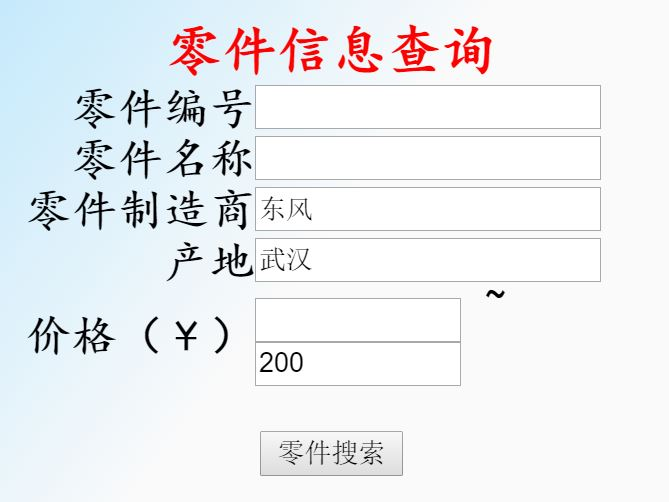
\includegraphics[width=0.7\linewidth]{figure/seniorPartSea}
\caption{高级零件查询示例}
\label{fig:seniorPartSea}
\end{figure}

\begin{figure}[H]
\centering

\includegraphics[width=0.9\linewidth]{figure/seniorPartRes}
\caption{高级零件查询示例结果}
\label{fig:seniorPartRes}
\end{figure}

和简单模式一样,各个字段依然为模糊搜索。如果输入的价格不为数字(如图\ref{fig:seniorNumError}),同样会有弹框(如图\ref{fig:seniorNumErrorAlert})。

\begin{figure}[H]
\centering
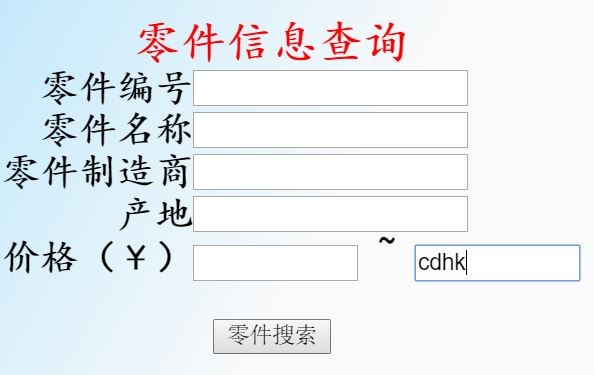
\includegraphics[width=0.7\linewidth]{figure/seniorNumError}
\caption{高级查询模式-价格格式错误}
\label{fig:seniorNumError}
\end{figure}

\begin{figure}[H]
\centering

\includegraphics[width=0.7\linewidth]{figure/seniorNumErrorAlert}
\caption{高级查询模式-价格错误弹窗}
\label{fig:seniorNumErrorAlert}
\end{figure}

\subsection{产品添加}
点击主页中\underline{添加产品},即可进入产品添加页面(如图\ref{fig:prod_add_index})。在页面中输入产品编号	 、产品型号、产品名称、产品制造商、产品产地和产品价格,所有项目为必填项,否则会弹框提醒(如图\ref{fig:error_noComplete}和\ref{fig:error_noComplete_alert})。此外价格必须为数字,否则也会报错(如图\ref{fig:prod_add_price_error}和\ref{fig:prod_add_price_error_alert})。
\begin{figure}[H]
\centering
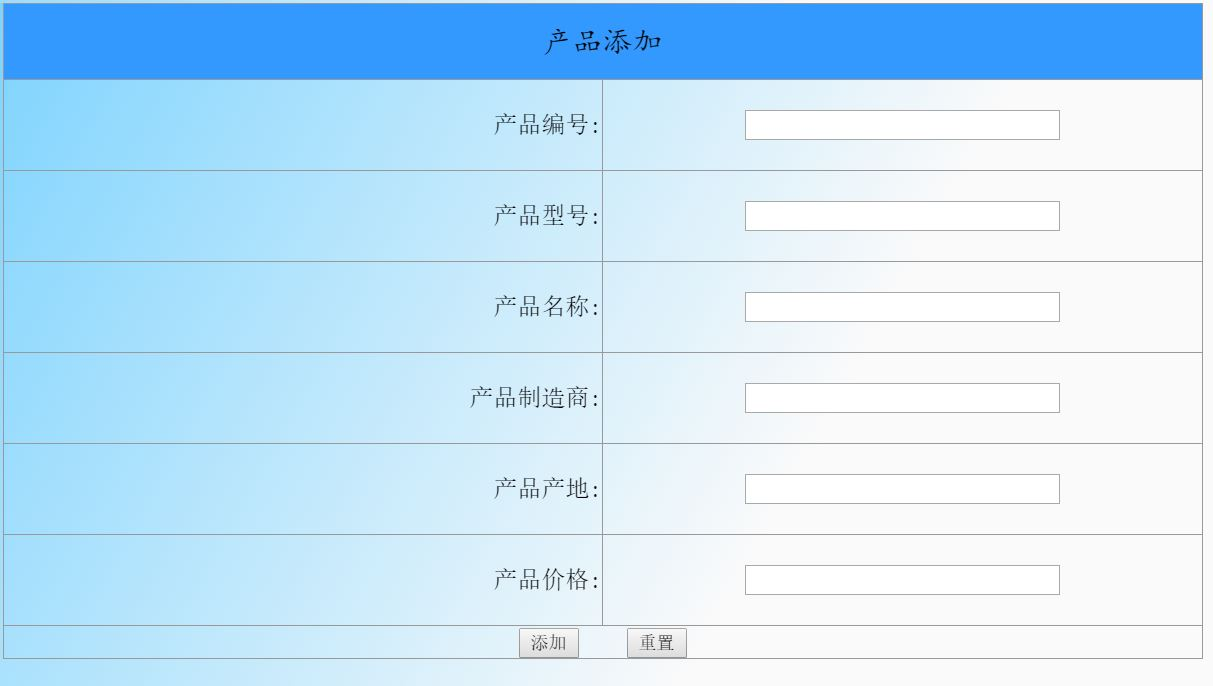
\includegraphics[width=0.8\linewidth]{figure/prod_add_index}
\caption{产品添加页面}
\label{fig:prod_add_index}
\end{figure}

\begin{figure}[H]
\centering
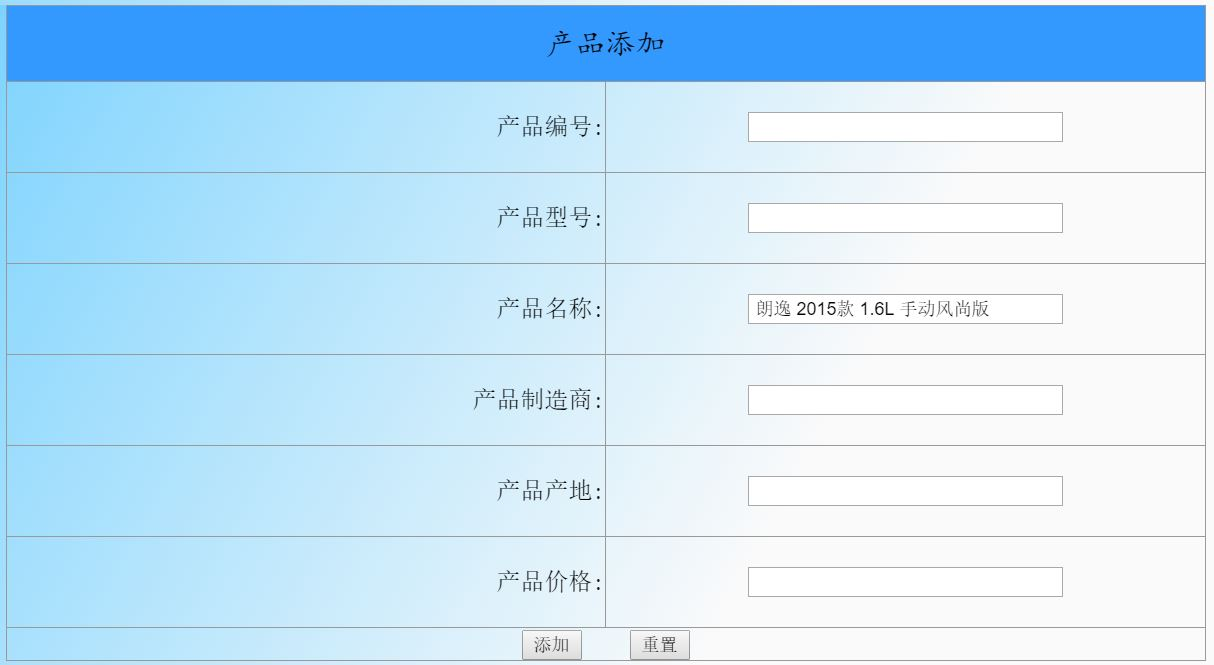
\includegraphics[width=0.8\linewidth]{figure/error_noComplete}
\caption{产品信息不完整}
\label{fig:error_noComplete}
\end{figure}

\begin{figure}[H]
\centering
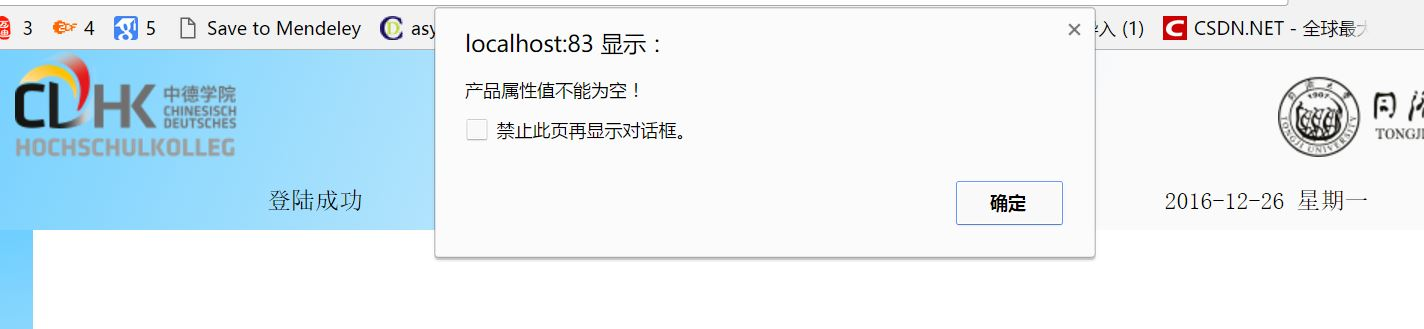
\includegraphics[width=0.8\linewidth]{figure/error_noComplete_alert}
\caption{产品信息不完整提示}
\label{fig:error_noComplete_alert}
\end{figure}

\begin{figure}[H]
\centering
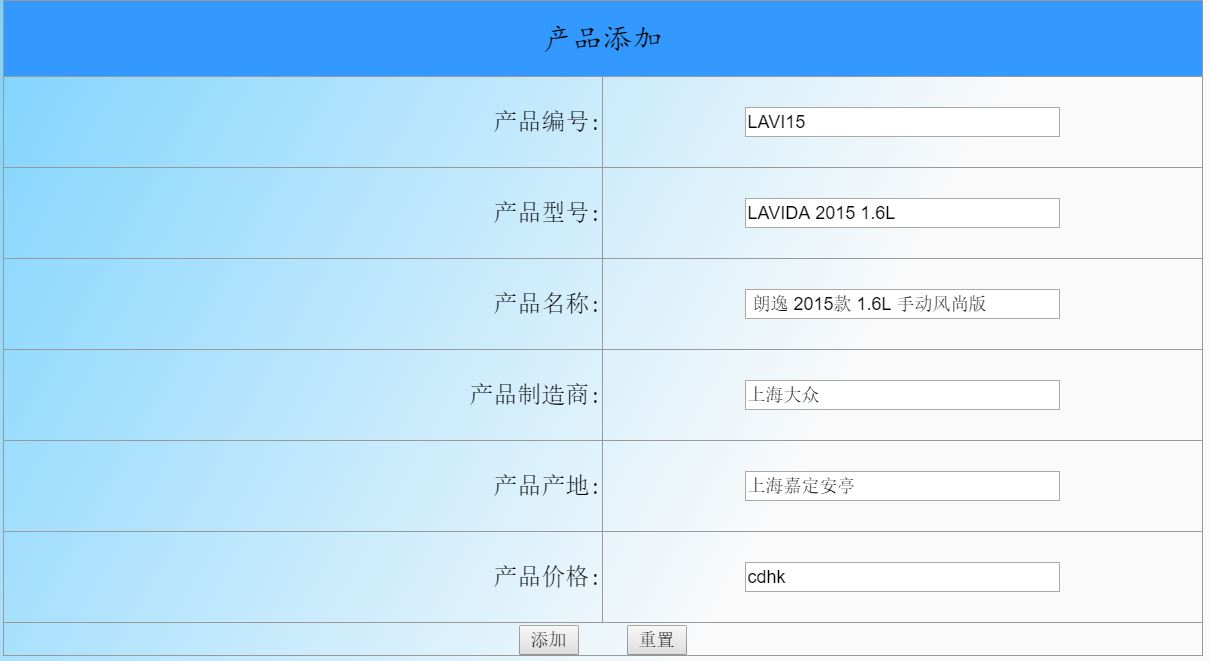
\includegraphics[width=0.8\linewidth]{figure/prod_add_price_error}
\caption{产品价格错误}
\label{fig:prod_add_price_error}
\end{figure}

\begin{figure}[H]
\centering
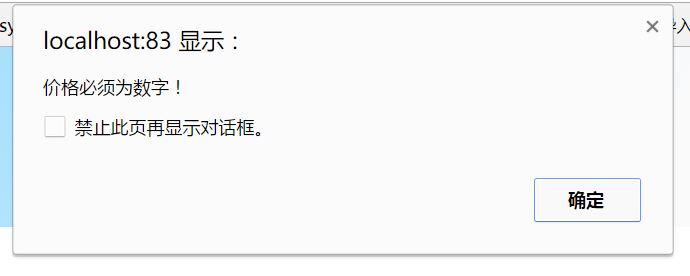
\includegraphics[width=0.8\linewidth]{figure/prod_add_price_error_alert}
\caption{产品价格错误提示}
\label{fig:prod_add_price_error_alert}
\end{figure}

在产品添加栏输入网址信息且保证价格为数字(如图\ref{fig:prod_add_sucess_inf}),点击\underline{添加},弹出添加成功提示(如图\ref{fig:prod_add_sucess})。
\begin{figure}[H]
\centering
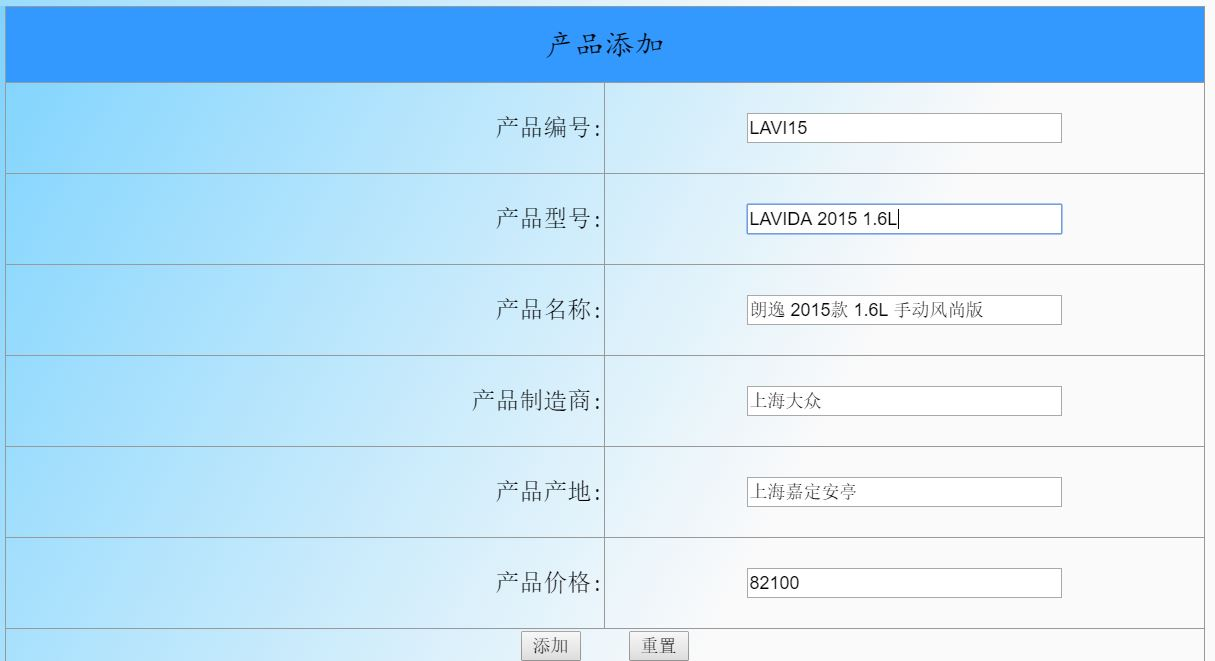
\includegraphics[width=0.8\linewidth]{figure/prod_add_sucess_inf}
\caption{产品信息完整且价格格式正确}
\label{fig:prod_add_sucess_inf}
\end{figure}
\begin{figure}[H]
\centering
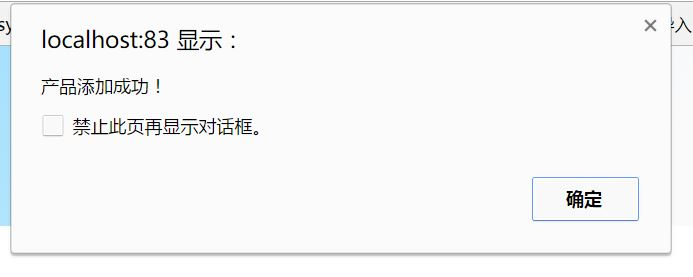
\includegraphics[width=0.8\linewidth]{figure/prod_add_sucess}
\caption{产品添加成功}
\label{fig:prod_add_sucess}
\end{figure}

\subsection{零部件添加}
点击主页中\underline{添加零部件},即可进入零部件添加页面,如图\ref{fig:part_add_index}。零部件所属产品型号是已经添加了的产品,拉下拉菜单可选择相应所属产品的型号,如选择New Passat 280TSI DSG。在这个页面中可添加零部件编号、零部件名称、零部件制造商、零部件产地和零部件价格,和产品添加一页面一样,这些项目都是必填字段,否则会弹出提醒``属性值不能为空'',其中价格必须为数字,否则也会弹框提醒。
\begin{figure}[H]
\centering
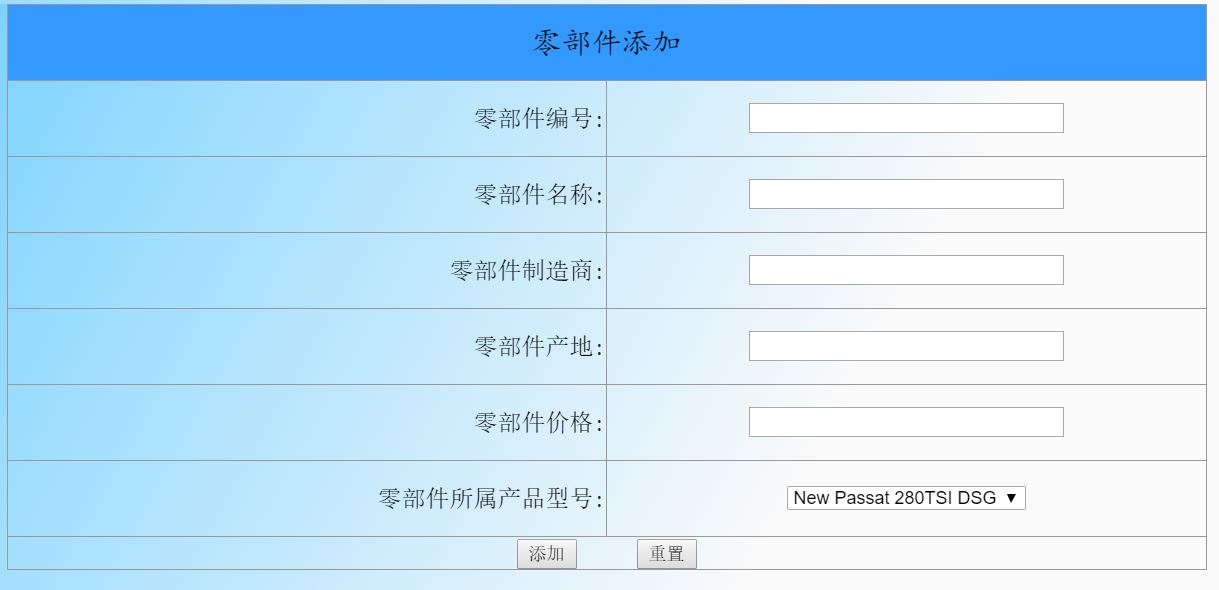
\includegraphics[width=0.9\linewidth]{figure/part_add_index}
\caption{零部件添加页面}
\label{fig:part_add_index}
\end{figure}

比如在页面中输入如图\ref{fig:part_add_inf}所示的零件信息,并且在下拉菜单中选择对应的产品型号。点击\underline{添加}按钮,即弹出添加成功提示d对话框\ref{fig:par_add_success},点击\underline{确认},回到零件添加页面\ref{fig:part_index1}。

\begin{figure}[H]
\centering
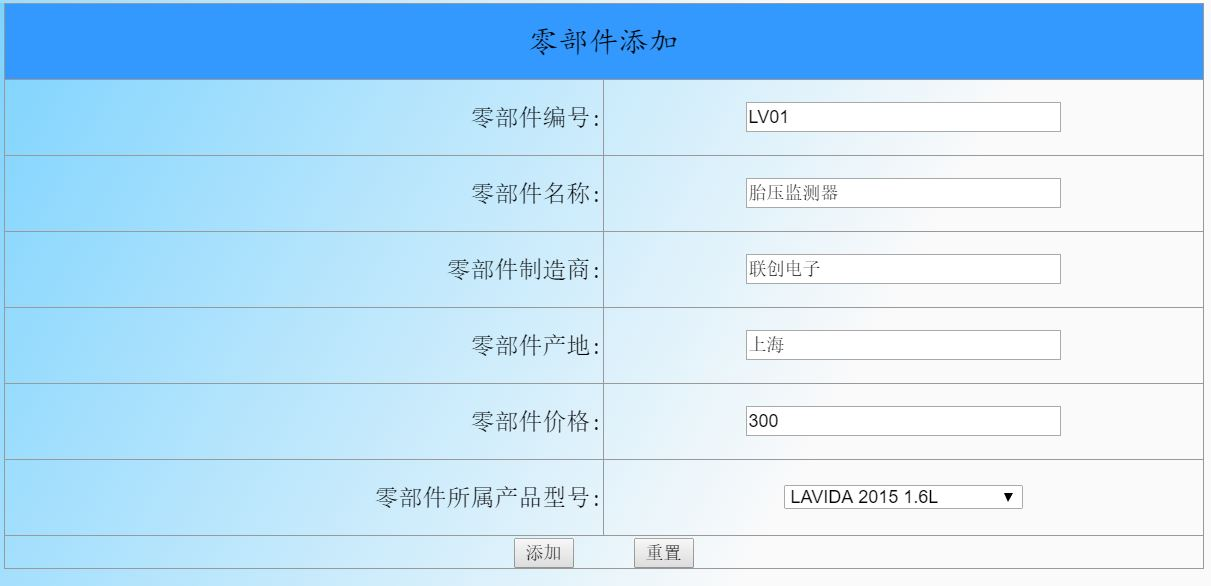
\includegraphics[width=0.8\linewidth]{figure/part_add_inf}
\caption{添加零部件}
\label{fig:part_add_inf}
\end{figure}

\begin{figure}[H]
\centering

\includegraphics[width=0.9\linewidth]{figure/par_add_success}
\caption{零部件添加成功}
\label{fig:par_add_success}
\end{figure}

\begin{figure}[H]
\centering
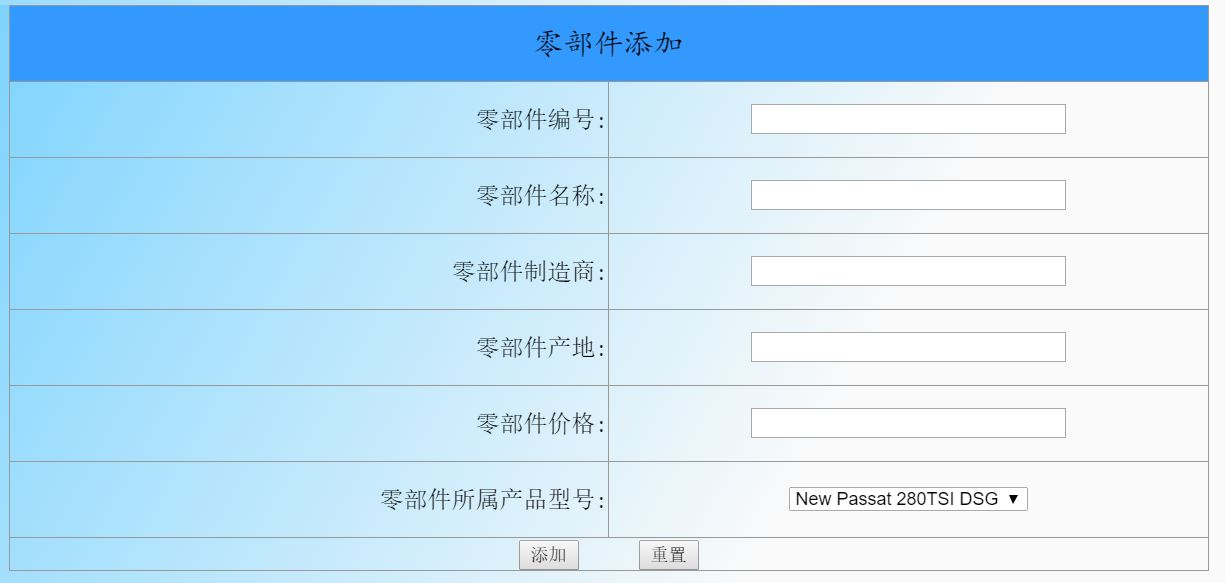
\includegraphics[width=0.8\linewidth]{figure/part_index1}
\caption{零件添加页面}
\label{fig:part_index1}
\end{figure}

\subsection{附属零件信息显示}
在产品查询页面中,输入查询条件,完成查询,将在界面上显示了产品查询结果,如图\ref{fig:spsearch_prd_name_result}所示。产品结果以表格形式给出,每一行代表一个产品记录,点击每一行后的\underline{零件信息},即可显示零件信息,图\ref{fig:POLO_part_infDetail}为汽车产品POLO 1.4L在MySQL数据库中的附属零件信息。
\begin{figure}[H]
\centering
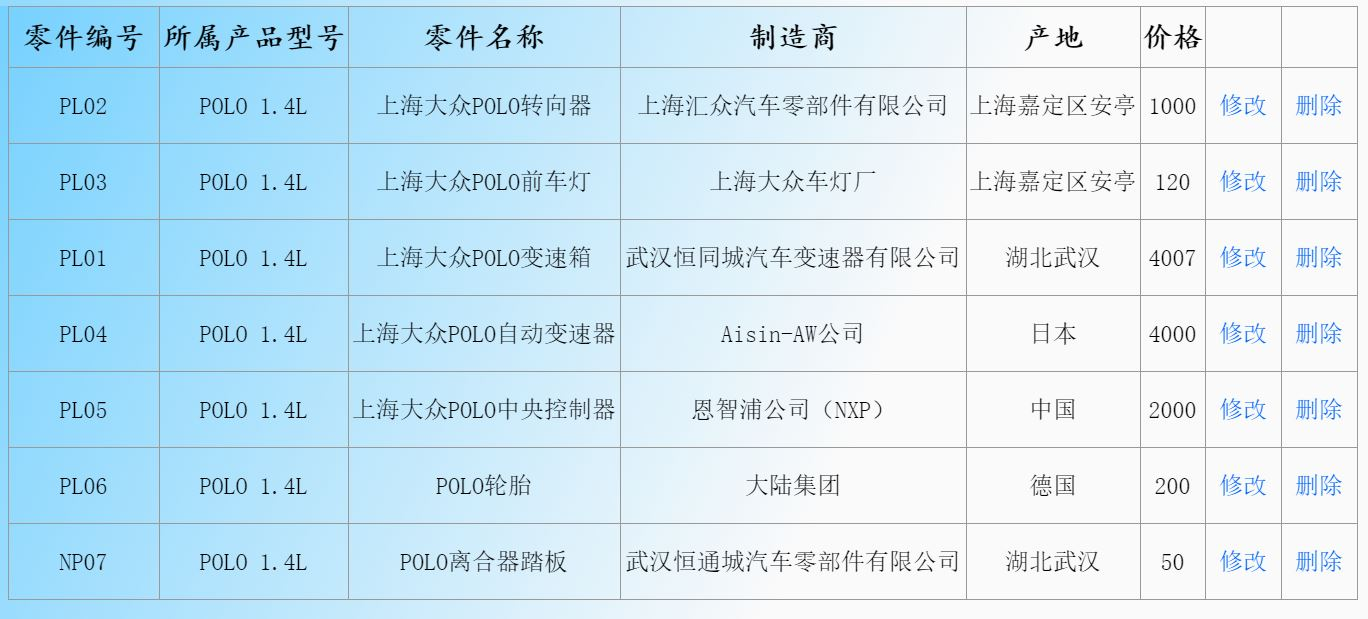
\includegraphics[width=0.8\linewidth]{figure/POLO_part_infDetail}
\caption{POLO 1.4L附属零件信息}
\label{fig:POLO_part_infDetail}
\end{figure}

在``删除后的产品记录''中也\underline{零件信息}链接;通过BOM表产品链接中也可以进入对应产品记录页面,该页面中同样也有\underline{零件信息}链接。
\subsection{记录删除}
本系统支持产品记录和零件的删除,系统在数据库建模时,将汽车产品和零部件的关系定义为``一对多''的关系,且支持外键约束,\textbf{即当用户将汽车产品删除后,对应的零件将全部自动删除},这一点用户需要注意。

在产品查询页面中,输入查询条件产品型号:LAVIDA 2016 1.6L,完成查询,将在界面上显示了产品查询结果,如图\ref{fig:LV16_prd_inf}所示。产品结果以表格形式给出,每一行代表一个产品记录,点击\underline{零件信息},LAVIDA 2016 1.6L的零件信息如图\ref{fig:LV16_prd_part_inf}所示,
\begin{figure}[H]
\centering
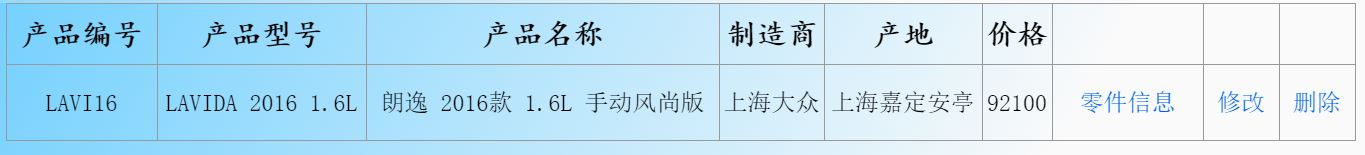
\includegraphics[width=0.9\linewidth]{figure/LV16_prd_inf}
\caption{LAVIDA 2016 1.6L}
\label{fig:LV16_prd_inf}
\end{figure}

\begin{figure}[H]
\centering
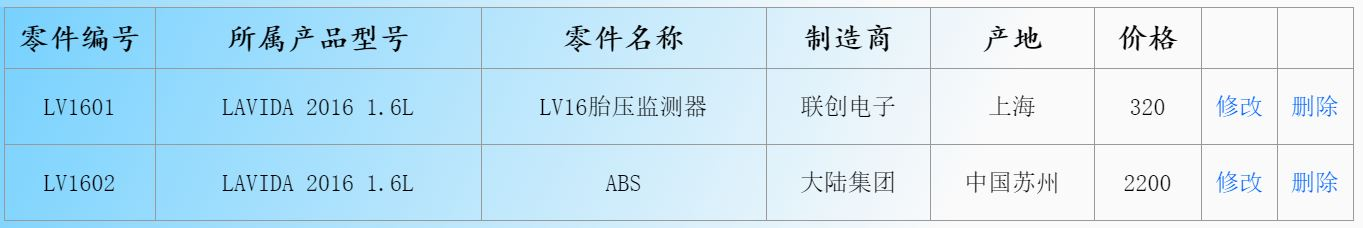
\includegraphics[width=0.9\linewidth]{figure/LV16_prd_part_inf}
\caption{LAVIDA 2016 1.6L 零件信息}
\label{fig:LV16_prd_part_inf}
\end{figure}


点击LAVIDA 2016 1.6L所在行后的\underline{删除}链接,即可删除汽车产品。同时其附属零件也将自动删除。为了防止误删,在点击删除后会弹出提醒对话框如图\ref{fig:prd_delete_alert},点击\underline{确认},将弹出删除成功对话框如图\ref{fig:prd_delete_success_alert},接着点击\underline{确认},即可显示删除之后,数据库中的产品记录如图\ref{fig:prd_deleteLV16}。其附属零件也将删除。
\begin{figure}[H]
\centering
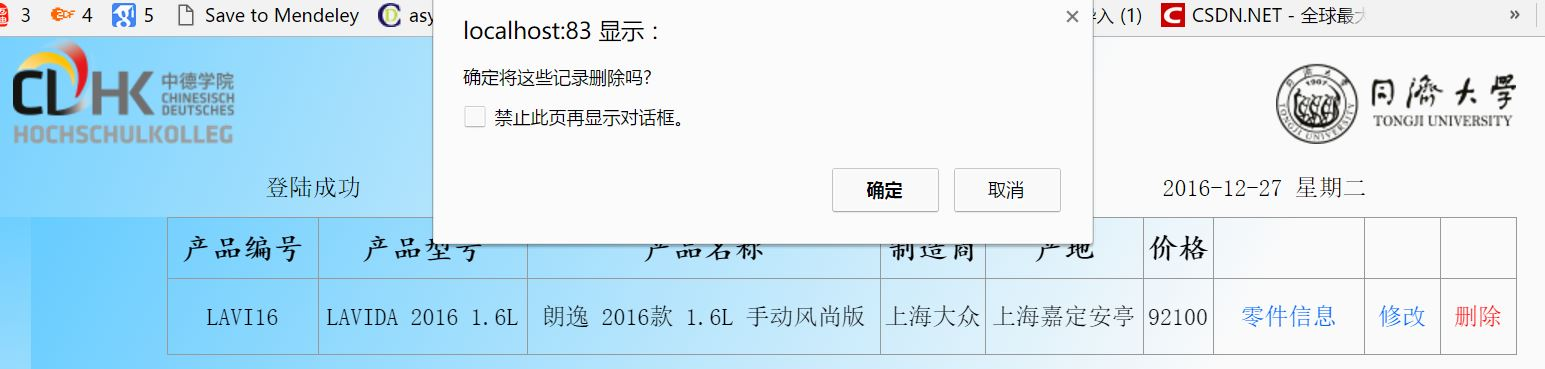
\includegraphics[width=0.8\linewidth]{figure/prd_delete_alert}
\caption{产品删除提醒对话框}
\label{fig:prd_delete_alert}
\end{figure}

\begin{figure}[H]
\centering
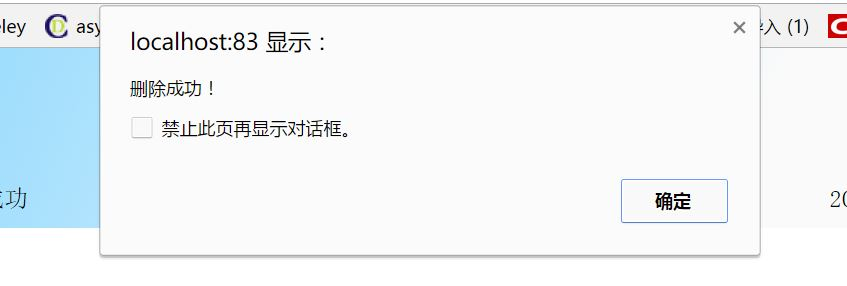
\includegraphics[width=0.7\linewidth]{figure/prd_delete_success_alert}
\caption{删除成功对话框}
\label{fig:prd_delete_success_alert}
\end{figure}

\begin{figure}[H]
\centering
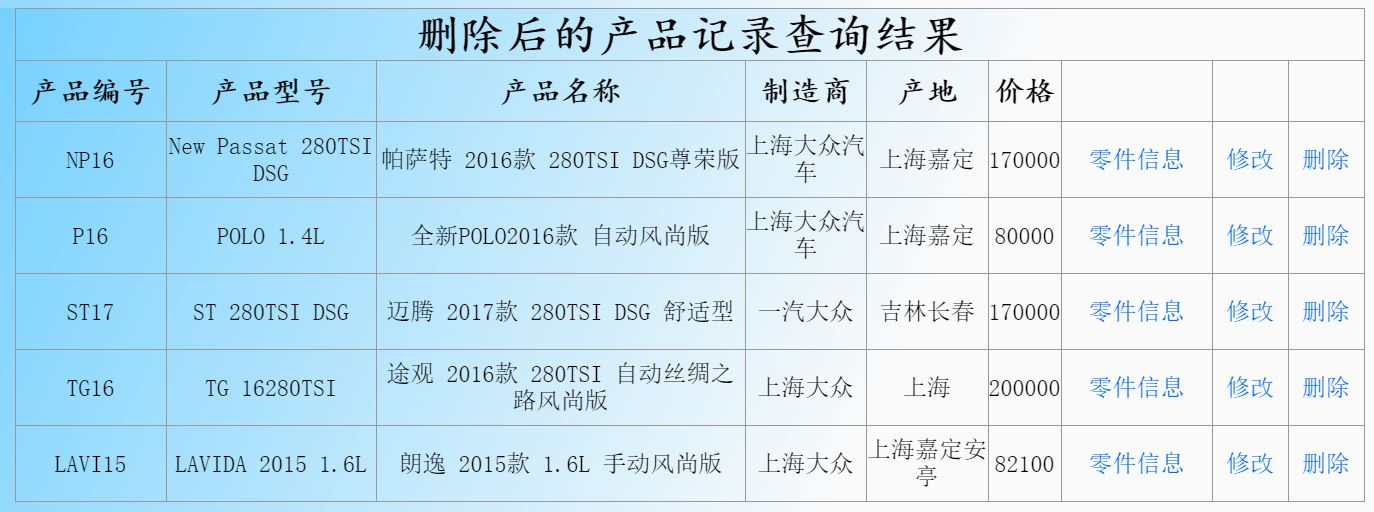
\includegraphics[width=0.8\linewidth]{figure/prd_deleteLV16}
\caption{删除之后的产品记录}
\label{fig:prd_deleteLV16}
\end{figure}

在零件查询页面中,输入查询条件零件名词\underline{轮胎}(图\ref{fig:part_delete_cond}),完成查询,将在界面上显示了零件查询结果,如图\ref{fig:part_delete_inf}所示。产品结果以表格形式给出,每一行代表一个零件记录,点击每一行后的\underline{删除信息},即可删除零件。为了防止误删,同样会弹出提醒对话框\ref{fig:part_delete_alert}。点击\underline{确认},将弹出删除成功对话框如图\ref{fig:part_delete_alert_success},接着点击\underline{确认},回到零件查询页面如图\ref{fig:part_delete_search_index},可以继续查询零件,并删除。
\begin{figure}[H]
\centering
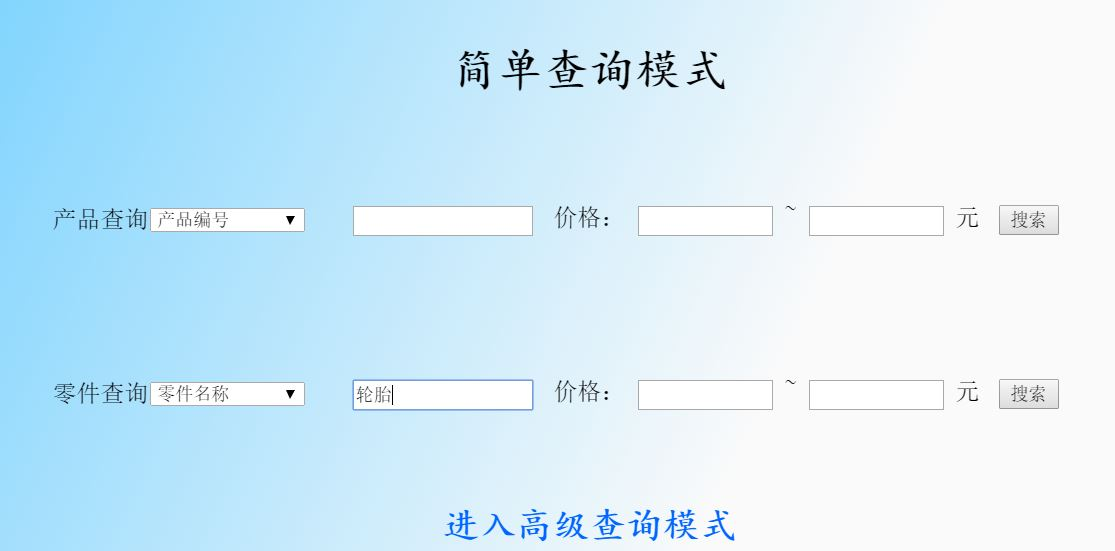
\includegraphics[width=0.8\linewidth]{figure/part_delete_cond}
\caption{查询待删除零件}
\label{fig:part_delete_cond}
\end{figure}

\begin{figure}[H]
\centering
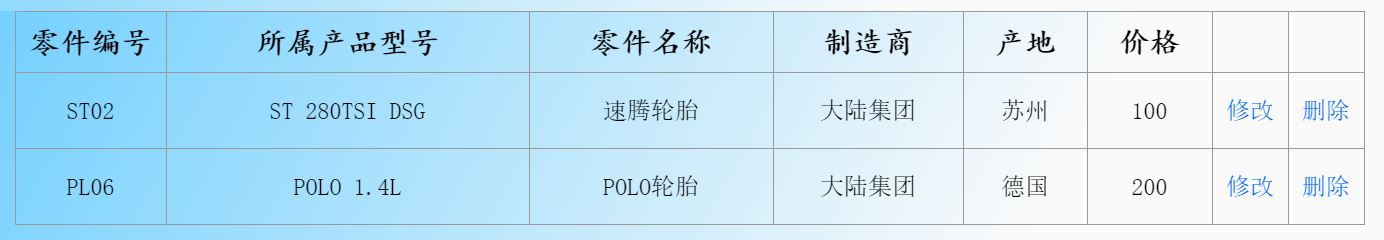
\includegraphics[width=0.8\linewidth]{figure/part_delete_inf}
\caption{待删除零件}
\label{fig:part_delete_inf}
\end{figure}

\begin{figure}[H]
\centering
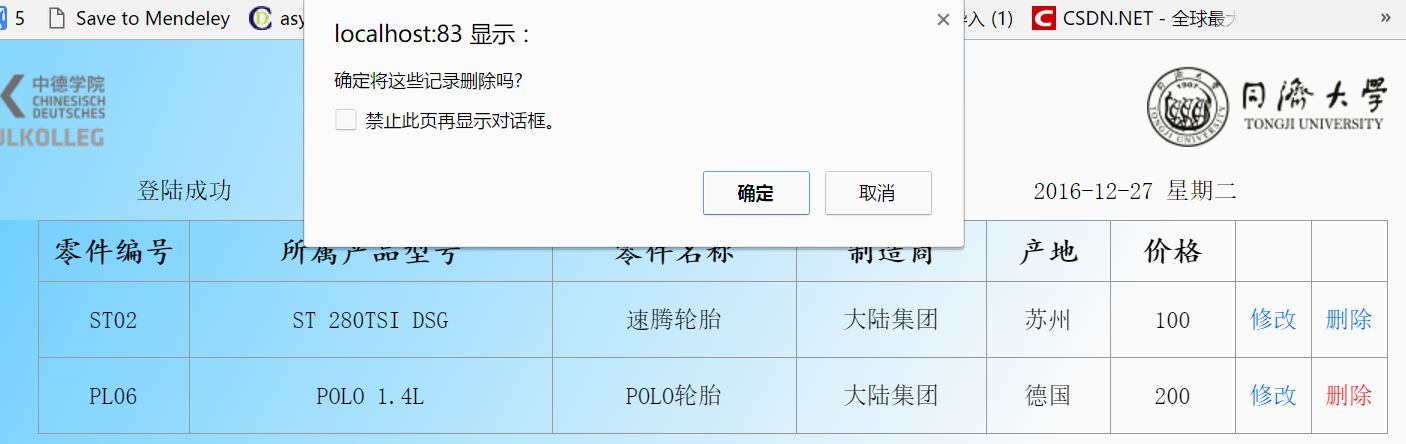
\includegraphics[width=0.8\linewidth]{figure/part_delete_alert}
\caption{零件删除提醒}
\label{fig:part_delete_alert}
\end{figure}

\begin{figure}[H]
\centering
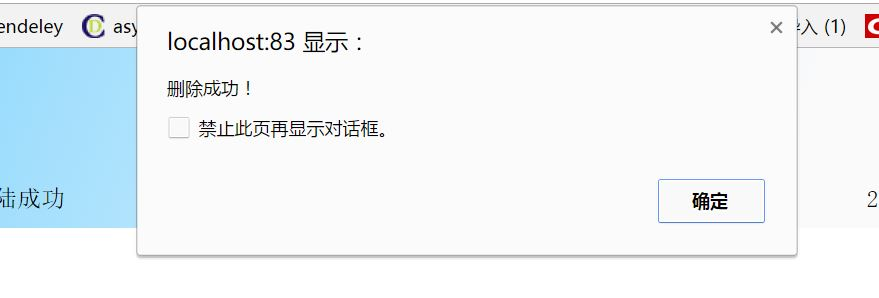
\includegraphics[width=0.8\linewidth]{figure/part_delete_alert_success}
\caption{零件删除成功}
\label{fig:part_delete_alert_success}
\end{figure}

\begin{figure}[H]
\centering
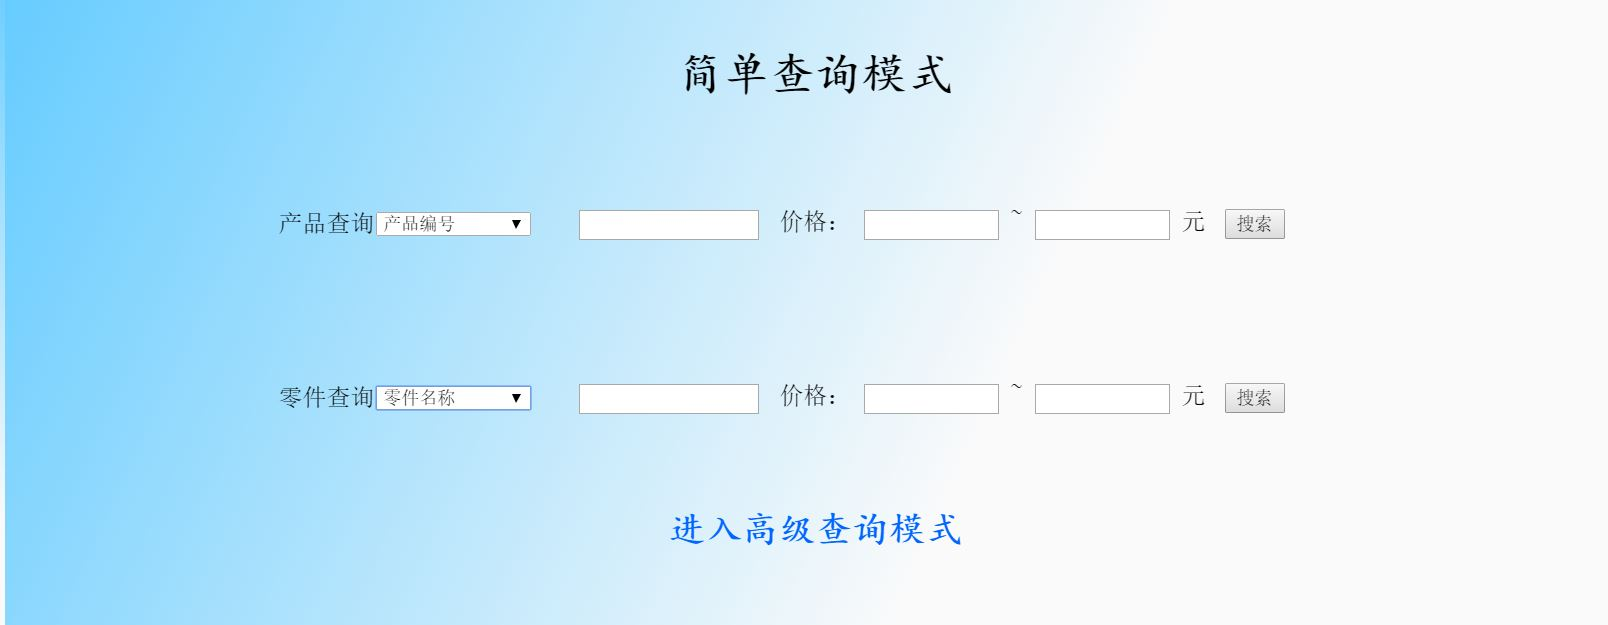
\includegraphics[width=0.8\linewidth]{figure/part_delete_search_index}
\caption{零件查询主页}
\label{fig:part_delete_search_index}
\end{figure}

本系统中,所有以表格形式显示产品和零件记录的页面均支持产品和零件的删除。
\subsection{记录修改}
和记录的删除一样,本系统中,所有以表格形式显示产品和零件记录的页面均支持产品和零件的修改。

在产品信息查询页面中,输入条件产地:上海,查询结果如图\ref{fig:prd_modify_recd},点击第一条记录后的\underline{修改}链接,进入产品修改页面\ref{fig:prd_mofify_index}。可以修改任意字段值,比如将产地修改为``上海市嘉定区安亭镇'',如图\ref{fig:prd_mofify_area}。点击\underline{提交}按钮,将弹出修改提醒对话框\ref{fig:prd_mofify_alert},点击\underline{确认},弹出产品修改成功对话框\ref{fig:prd_mofify_success},接着点击\underline{确认},显示修改后的产品信息(图\ref{fig:prd_modify_success_1}),可以继续修改。零件所属产品只能在已添加的产品记录中选择。
\begin{figure}[H]
\centering
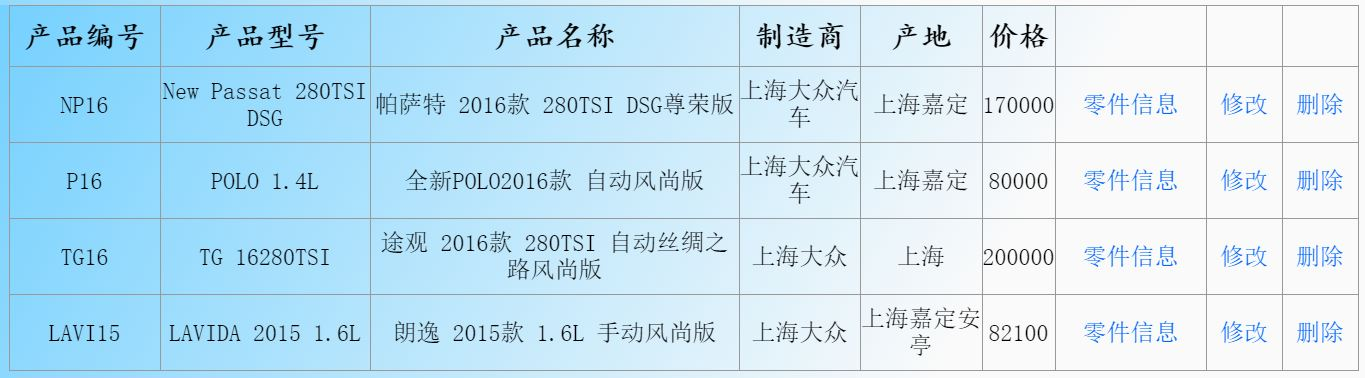
\includegraphics[width=0.8\linewidth]{figure/prd_modify_recd}
\caption{待修改产品}
\label{fig:prd_modify_recd}
\end{figure}

\begin{figure}[H]
\centering
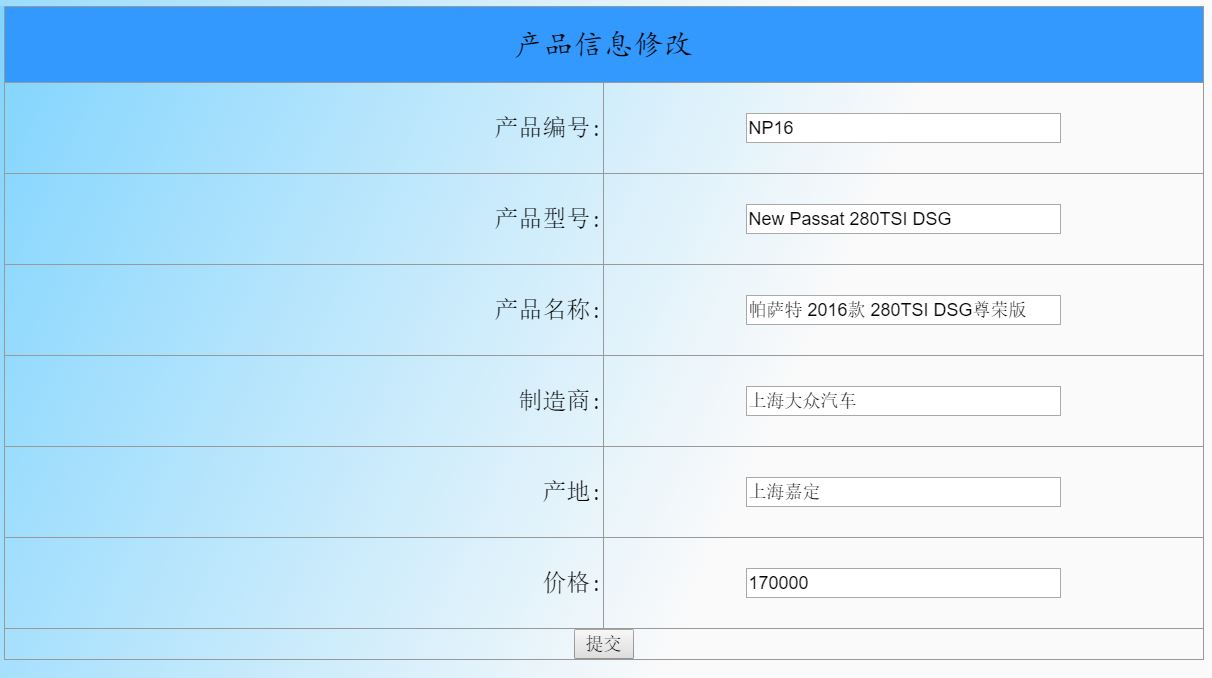
\includegraphics[width=0.8\linewidth]{figure/prd_mofify_index}
\caption{产品修改页面}
\label{fig:prd_mofify_index}
\end{figure}

\begin{figure}[H]
\centering
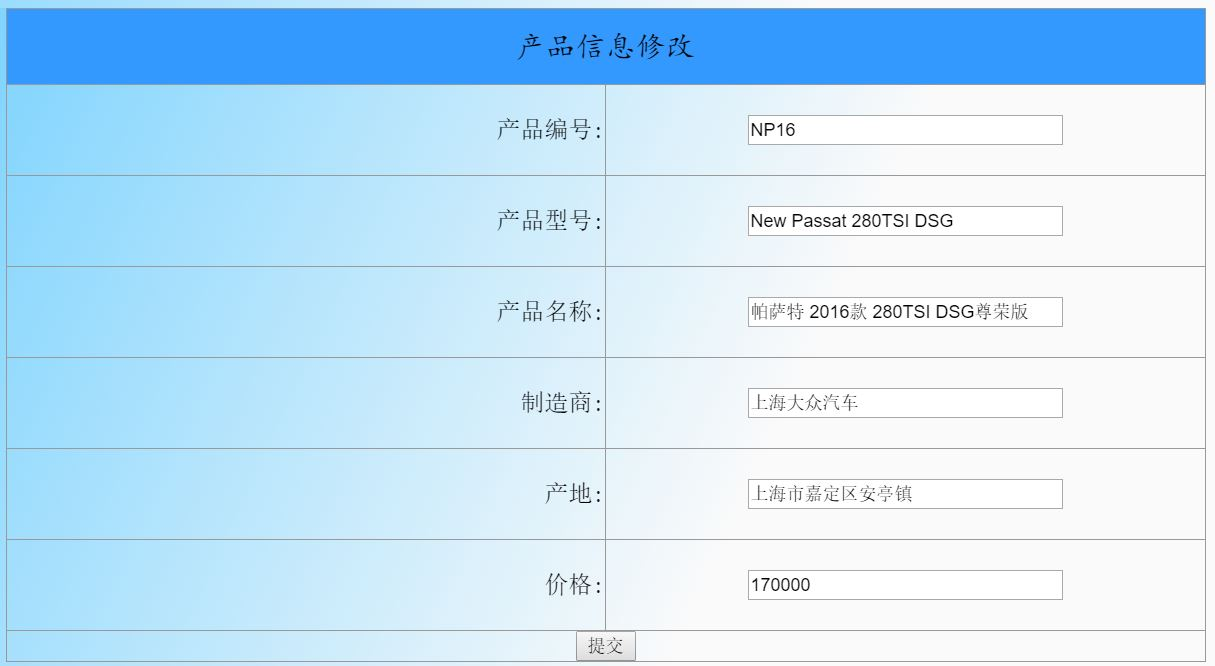
\includegraphics[width=0.8\linewidth]{figure/prd_mofify_area}
\caption{修改产品产地}
\label{fig:prd_mofify_area}
\end{figure}

\begin{figure}[H]
\centering
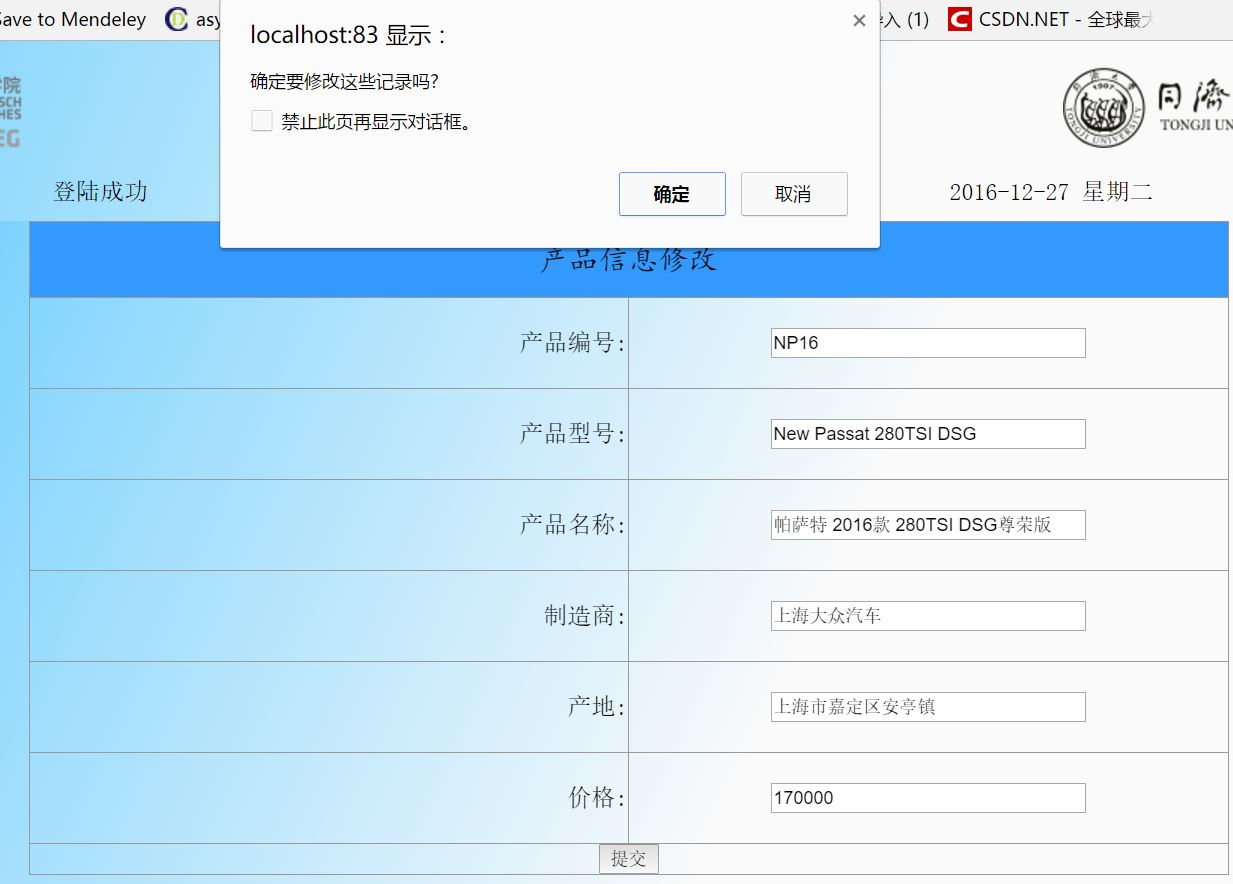
\includegraphics[width=0.8\linewidth]{figure/prd_mofify_alert}
\caption{产品修改提醒}
\label{fig:prd_mofify_alert}
\end{figure}

\begin{figure}[H]
\centering
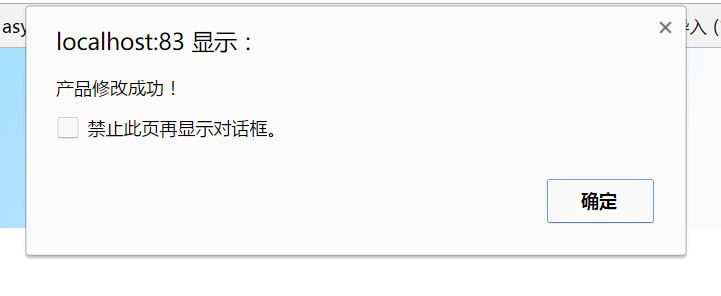
\includegraphics[width=0.8\linewidth]{figure/prd_mofify_success}
\caption{产品修改成功}
\label{fig:prd_mofify_success}
\end{figure}

\begin{figure}[H]
\centering
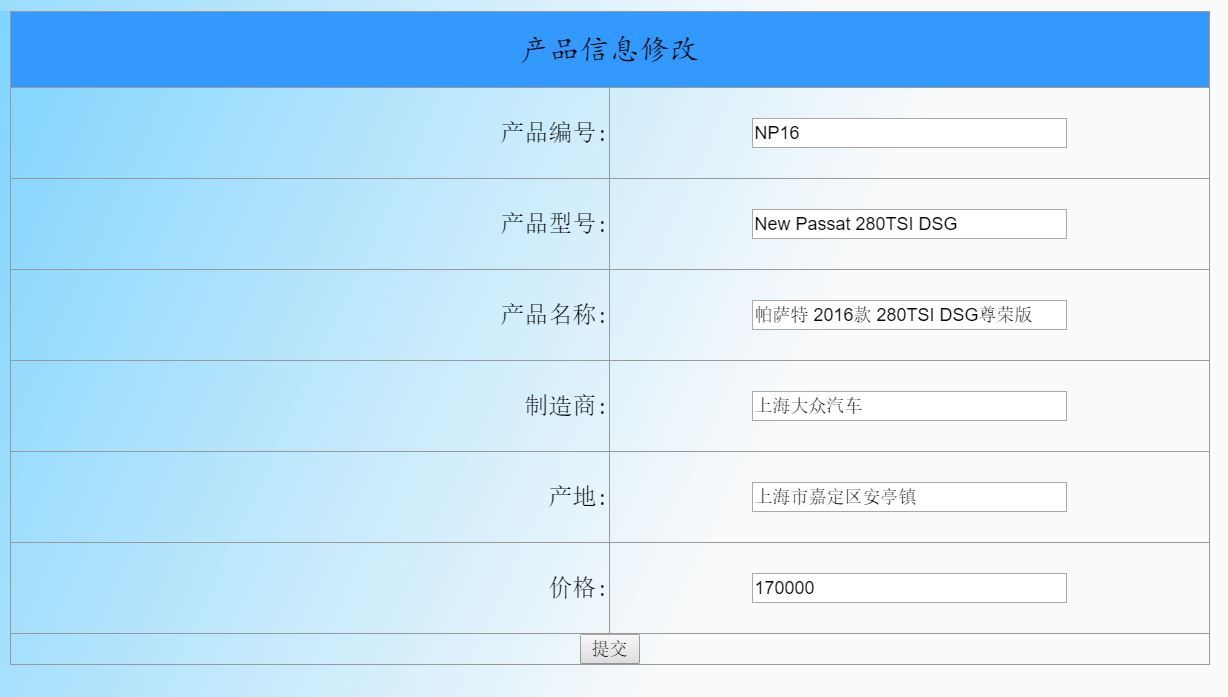
\includegraphics[width=0.8\linewidth]{figure/prd_modify_success_1}
\caption{修改后的产品记录}
\label{fig:prd_modify_success_1}
\end{figure}

在零件信息查询页面中,输入条件产地:武汉,查询结果如图\ref{fig:part_modify_inf},点击``离合器''记录后的\underline{修改}链接,进入零件修改页面\ref{fig:part_modify_index}。可以修改任意字段值,比如将产品名词修改为``ST离合器'',如图\ref{fig:part_modify_name}。点击\underline{提交}按钮,将弹出修改提醒对话框\ref{fig:part_modify_alert},点击\underline{确认},弹出零件修改成功对话框\ref{fig:part_modify_success},接着点击\underline{确认},显示修改后的零件信息(图\ref{fig:part_modify_success1}),可以继续修改。零件所属产品只能在已添加的产品记录中选择。
\begin{figure}[H]
\centering
\includegraphics[width=0.8\linewidth]{figure/part_modify_inf}
\caption{待修改零件信息}
\label{fig:part_modify_inf}
\end{figure}

\begin{figure}[H]
\centering
\includegraphics[width=0.8\linewidth]{figure/part_modify_index}
\caption{零件信息修改主页}
\label{fig:part_modify_index}
\end{figure}

\begin{figure}[H]
\centering
\includegraphics[width=0.8\linewidth]{figure/part_modify_name}
\caption{修改零件名称}
\label{fig:part_modify_name}
\end{figure}

\begin{figure}[H]
\centering
\includegraphics[width=0.8\linewidth]{figure/part_modify_alert}
\caption{零件修改提醒}
\label{fig:part_modify_alert}
\end{figure}

\begin{figure}[H]
\centering
\includegraphics[width=0.8\linewidth]{figure/part_modify_success}
\caption{零件信息修改成功}
\label{fig:part_modify_success}
\end{figure}

\begin{figure}[H]
\centering
\includegraphics[width=0.8\linewidth]{figure/part_modify_success1}
\caption{修改后的零件信息}
\label{fig:part_modify_success1}
\end{figure}

